\documentclass[a4paper,14pts]{report}
\usepackage{settings-my-thesis}
\includeonly{ introduzione/intro,%
               %capitoli/capitolo-1,%
               capitoli/capitolo-2,%
               %capitoli/capitolo-3,%
              }
\begin{document}
\titlepage{

\includegraphics[keepaspectratio]{logoSapienza}
\\
\vspace{150pt}
\begin{center}
{\onehalfspacing
\huge{\textcolor{Mahogany!80!Mulberry}{\textsf{Uno Schema Semi-Lagrangiano per il Moto per Curvatura Media che preserva il Volume}}}}
\end{center}
\vspace{150pt}
\begin{flushleft}
{\small\textcolor{Mahogany!80!Mulberry}{\textsf{Facoltà di Scienze Matematiche Fisiche e Naturali}\\
\textsf{Corso di Laurea Magistrale in Matematica per le Applicazioni}}\\
\textsf{Michele Cipolla\\
n$^{\circ}$ matricola 1174687}}
\end{flushleft}
\vspace{50pt}
\begin{flushleft}
{\small\textsf{Relatrice:\\
Prof.Elisabetta Carlini}\\
\bigskip
\textsf{Anno Accademico 2013/2014}
}
\end{flushleft}}

\cleardoublepage
\pdfbookmark{\contentsname}{Contents}
\tableofcontents
\cleardoublepage
\phantomsection
\addcontentsline{toc}{chapter}{Elenco delle figure}
\listoffigures
\chapter*{Introduzione}
\phantomsection
\addcontentsline{toc}{chapter}{Introduzione}

Un campo della matematica che in questi anni si sta sviluppando
notevolmente, è quello che si occupa del trattamento delle immagini
sia 2D che 3D. Se da un lato sono migliorati gli strumeti di
acquisizione delle stesse (come  scanner 2D/3D), dall'altro si sta
sviluppando sempre più l'idea, già da anni consolidata, di utilizare
equazioni alle derivate parziali (PDE) nel trattamento delle
immagini. L'idea si basa sul concetto di \emph{scale-space} o
\emph{rappresentazione multiscala}, in cui l'immagine
iniziale $u_0(x)$ viene racchiusa in una famiglia $u(x,t)$, con
$t\in\mathbb{R}^+$ parametrizzante la scala, attraverso l'azione di un
\emph{kernel} (filtro) $K(\cdot,t)$. Uno dei filtri più
usati  e studiati è quello \emph{gaussiano}, in questo caso  $u(x,t)$
è definita dalla convoluzione del filtro con $u_0(x)$ e può essere
vista come la soluzione dell'equazione del calore con dato iniziale $u_0(x)$
\[
u_t=\Delta u.
\]
Quindi il fatto chiave è che uno \emph{scale-space} può essere
ottenuto come una soluzione di un'equazione di evoluzione alle
derivate parziali. 
%le proprità principali, la linearità e la \emph{cusualità}, cioè
%non viene aggiunta  ``informazione'' quando ci spostiamo da una scala
%$t_1$ ad una $t_2>t_1$, che matematicamente può essere tradotto con il
%principio del massimo ed  è anche legata alla proprietà di
%\emph{semi-gruppo}, vale a dire che $u(x,t_2)$ può essere ottenuta da
%$u(x,t_1)$ senza conoscere $u_0(x)$, con $t_1<t_2$.   Nonostante queste
%buone proprietà, tuttavia, il flusso calorico classico presenta alcuni
%problemi, in particolare non è intrinseco alla giometria
%dell'immagine. Questo problema è stato risolto
%(\cite[][]{sapiro:tann}) sostituendo il flusso calorico classico con
%un flusso  geometrico, che in generale dipende da caretteristiche
%geometriche dell'oggetto in esame come ad esempio la curavtura. Uno
%\emph{scale-space} che si evolve secondo questi flussi, essendo
%ottenuto come soluzione di un PDE, continua a soddisfare le proprietà
%di causualità (principio del massimo) e di semi gruppo ed in più è
%intrinseco alle proprietà dell'oggetto in esame. 
Questo concetto è alla base di molte applicazioni nella computer
grafica e nell'analisi dell'immagini, in modo particolare può essere
usato per processi di \emph{denoising} di un immagine. E' noto che
quando acquisiamo o inviamo un immagine questa si può deteriorare, cioè 
viene aggiunto del \emph{rumore}, e quindi abbiamo bisogno di
filtrarla per eliminare le discontinuità. Il modello di filtraggio per
immagini 3D che presentiamo in questo lavoro, si basa su uno dei flussi più
studiati nella letteratura, il flusso per curvatura media. Questo,
tuttavia presenta dei limiti, in quanto è stato dimostrato che
superfici convesse evolvono in un punto, mentre superfici
non convesse posso subire dei cambiamenti topologici generando delle
singolarità. Il colasso in un punto è, come si può intuire, un aspetto
limitante nel denoising soprattutto quando abbiamo a che fare con
rumore che per essere eliminato necessita di molte iterazioni
di filtraggio. Nel lavoro di Sapiro \cite[][]{gui:sapiro}, il
flusso per curvatura media è stato riscritto in modo tale da
conservare il volume. Tramite la rappresentaizone 
\emph{level-set} delle superfici introdotta da Oscher e Sethian,
abbiamo riscritto l'equazione per curvatura media che preserva il
volume ottenendo un PDE parabolico non lineare del secondo ordine
singolare nei punti dove il gradiente della soluzione si annulla, con
il flusso formato da due termini di cui uno descrive l'evoluzione 
per curvatura media e l'altro è un termine di trasporto che conserva
il volume. Quindi è stato necessario immergere il tutto nella teoria
delle soluzioni viscose; anche se, eccezion fatta per alcuni casi
particolari, ancora non sono stati raggiunti risultati definitivi
sull'esistenza e unicità delle soluzioni nel caso della nostra
equazione. Discretizzando tale equazione con uno schema
Semi-Lagrangiano e un schema \emph{ad hoc} nel caso di gradiente 
nullo abbiamo ralizzato un algoritmo di filtraggio (scritto
in\emph{C-Language}) che preserva il volume. Abbiamo iniziato a
testarlo sull'evoluzione di superfici geometriche, prive di rumore,
confrontandolo con lo schema MCM e verificando che il volume viene
preservato. Una volta constatato il correto funzionamento del metodo,
siamo passati al filtraggio di superfici 3D, su cui è stato aggiunto
del rumore, simulato sia con una distribuzione gaussiana (tecnica
standard) sia con una funzione che aggiunge dei dischi di rumore
random. Nel caso di superfici geometriche, si riesce a ripulire la
figura superando i limiti dello schema classico, tra cui il collasso
in un punto di superfici convesse ed a ritardare i cambiamenti topologici che
emergono per quelle non convesse, come nel caso del manubrio; mentre
sono rimasti i fenomeni di smussamento dei contorni tipici di MCM.
Nel caso dell'immagine reale, su cui l'abbiamo testato, non sono
emerse troppe differenze a causa dell'impossibilità di effettuare troppe
iterazioni.
 
La tesi è strutturata come segue: nel Capitolo §\ref{cap:cap1} abbiamo
richiamato alcune nozioni sulle superfici in forma level-set,
presentato l'equazione di evoluzione per curvatura media, calcolato il
termine che ci conserva il volume e riscritto il tutto in formulazione
level-set. Nel Capitolo §\ref{cp:cp2}, abbiamo esposto i concetti
realitivi a soluzioni di viscosità, riportando alcuni teoremi di
esistenza e unicità in casi particolari, necessari per fornire un
robusto background teorico alla nostra equazione. Lo schema del moto
per curvatura media classico (MCM) e la sua versione che preserva il
volume (VPMCM) sono stati ottenuti nel Capitolo §\ref{cp:cp2-00},
riportando anche il conto per la consistanza di MCM e di una versione
semplificata di PVMCM. Infine nel Capitolo §\ref{cap:cp4} abbiamo
sia mostato il buon comportamento dello schema VPMCM nel caso di superfici
geometriche, sia in presenza che in assenza di rumore, e testato su di
un'immagine reale riportando le dovute considerazioni. 
   

\chapter{Evoluzione Geometrica Per Curvatura Media}
'WIP'
%%%%%%%%%%%%%%%%%%%%%%%%%%%%%%%%%%%%%%%%%%%%%%%%%%%%
%
% Section 1.1
%
%%%%%%%%%%%%%%%%%%%%%%%%%%%%%%%%%%%%%%%%%%%%%%%%%%%%
\section{Superfici in rappresentazione level-set}
\label{sec:cp1-00}
Un insieme $S\subset\mathbb{R}^3$ è chiamato superfice di classe $C^m$ (o ipersuperficie se siamo in $\mathbb{R}^N$ con $N>3$) intorno ad un punto $x_0$ di $S$ se esiste una funzione $u(x)$ di classe $C^m$ definita in un intorno $U$ di $x_0$ tale che
\[
S\cap U=\left\{x\in U; u(x)=0\right\}
\]
e il gradiente di $u$
\[
 Du=\left(\frac{\partial u}{\partial x_1},\dots,\frac{\partial u}{\partial x_3}\right)
\]
non svanisce su $S$. Tale rappresentazione è chiamta \emph{level-set}. Se $u$ può essere presa $C^{\infty}$ in $U$, diremo che la superficie $S$ è regolare intorno ad $x_0$ e se $u$ è anche definita intorno ad ogni punto di $x_0\in S$, allora si parla semplicemetne di superficie regolare. Questa rappresentazione può essere estesa anche ad insiemi dipendenti dal tempo. Difatti diremo che una famiglia $S_t$ è una superficie regolare che si evolve nel tempo se esiste una funzione $u(x.t)$ definita per ogni $x\in S_t$ e $t\in I$ tale che:
\[
S_t=\left\{x\in S_t; u(x,t)=0\right\},
\]
e tale che il gradiente spaziale di $u$ non svanisca su $S_t$.
\begin{osservazione}
 La superfice può essere rappresentata anche tramite cordinate locali. Un sottoinsieme $S\subset\mathbb{R}^3$ rappresenta una superficie intorno ad un punto $x_0$ di $S$, attraverso l'immagine $\varphi(U^{'})$ di una qualche mappa $\varphi$ di classe $C^m$ da un insieme aperto $U^{'}\subset\mathbb{R}^2$ in $\mathbb{R}^3$ con rango massimo, cioè la matrice Jacobiana $\nabla\varphi$ ha le colonne linearmenti indipendenti.
L'equivalenza tra le due rappresentazioni è garantita dal teorema della funzione implicita.
\end{osservazione} 

Supponiamo che $S$ sia una superfice intorno a $x_0\in S$. Un vettore $\tau\in\mathbb{R}^3$ è chiamato \emph{vettore tangente} di $S$ in $x_0$, se esiste una curva $\zeta\in C^1$ su $S$ tale che $\zeta = x_0$ e $d\zeta(t)/dt = \tau$ in $t=0$, dove $\zeta$ è definita almeno in un intorno di $0$. Lo spazio dei vettori tangenti in $x_0$ è chiamato \emph{spazio tangente} di $S$ in $x_0$ ed è denotato con $T_{x_0}S$. Un \emph{vettore unitario normale} $\vec{n}(x_0)$ in $x_0$ a $S$ è un vettore di $\mathbb{R}^3$ con norma uno ortogonale al $T_{x_0}S$, ed è unico a meno del segno. Se $\vec{n}(x)$ è un vettore normale unitario in $x$ vicino $x_0$ e esso dipende da $x$ in modo almeno continuo, diremo che $\vec{n}$ è un campo unitario normale di orientazione (attorno a $x_0$) di $S$. Vediamo che esiste almeno in un intorno di $x_0$. Per $x\in S\cap U$ sia $\zeta(t)$ una curva su $S$ tale che $\zeta(0)=x$. Deriviamo $u(\zeta(t)) = 0$ e cancoliamolo in $t=0$
\[
\left<Du(x),\frac{d\zeta}{dt}(0)\right> = 0.
\]
Questo ci dice che il gradiente in $x$ di $u$ è ortogonale al piano tangente a $S$ in $x$. Per la formulazione level-set $u\in C^m$ , $Du\in C^{m-1}$ ($m>0$) quindi almeno continua e $Du$ non svanisce intorno a $x_0$; quindi
\[
\vec{n}(x)=-\frac{Du(x)}{|Du(x)|},
\]
è un campo vettoriale unitario di orientazione intorno ad $x_0$. Il segno meno è per fissare le idee. Quindi lo spazio tangente per $x\in S$ intorno a $x_0$ è dato da
\[
T_xS = \left\{\tau\in\mathbb{R}^3;<\tau,\vec{n}(x)>=0\right\}.
\]

\begin{figure}[!hp]
  \tdplotsetmaincoords{60}{40}
  \begin{tikzpicture}[tdplot_main_coords,gray,thick]

    \coordinate (O) at (0,0,0);

    \tdplotsetcoord{P}{1.5}{90}{240};
    \tdplotsetcoord{P1}{2.5}{90}{105};
    \tdplotsetcoord{P2}{2.7}{90}{-30};
    \tdplotsetcoord{P3}{3.4}{90}{45}

    
    \draw[->,blue] (0,0,0)node[anchor=east]{$x$} -- 
    (2,0,0) node[anchor=south]{${\tau}^2$};
    \draw[->,blue] (0,0,0) -- (0,2,0) node[anchor=north]{${\tau}^1$};
    \draw[->,blue] (0,0,0) -- (0,0,2.5) node[anchor=north east]{$\vec{n}$};
    
    \draw (P) -- (P1) -- (P3) -- (P2) -- (P);
    
    \tdplotsetcoord{W}{6}{90}{281}
    \tdplotsetcoord{W1}{6.5}{90}{91}
    \tdplotsetcoord{W2}{6}{90}{318}
    \tdplotsetcoord{W3}{5.5}{90}{25}
    
    \draw (W) .. controls (-2,0,0) and (-2,1,0) .. (W1);
    \draw (W2) .. controls (3,0,0) and (3,0.5,0) .. (W3);
    \draw (W) to[out=60,in=60] (W2);
    \draw (W) to[out=240,in=240](W2);
    \draw (W1) to[out=190,in=190] (W3);
    \draw (W1) to[out=10,in=10] (W3);

  \end{tikzpicture}

  \caption{Piano tangente e versore normale alla superficie $S$ nel punto $x$.}
  \label{fig:cp-111}
\end{figure}

Sia $S$ una superfice in $\mathbb{R}^3$, per un punto $x_0$ sia $\tau$ un vettore tangente di $S$ in $x_0$ e sia $X$ un campo vettoriale $C^1$ su $S$ intorno a $x_0$. Qui $C^1$ vuol dire che può essere esteso ad una funzione $C^1$ in un intorno di $x_0$ in $\mathbb{R}^3$. Sia $\zeta$ una curva su $S$ tale che
\[
\zeta(0)=x_0,\quad\frac{d\zeta(t)}{dt}=\tau,
\]
la derivata tangenziale nella direzione $\tau$ è così definita
\[
(D_{\tau}X)(x_0)=\frac{d}{dt}\left(X(\zeta(t))\right)_{|_{t=0}}.
\]
Se $X$ è esteso in un intorno di $x_0$ in $\mathbb{R}^3$, allora essendo $C^1$ è ben definita la matrice $3\times 3$ jacobiana $\nabla X$, quindi
\begin{equation}
\label{eq:cp1-1-01}
(D_{\tau}X)(x_0)=(\tau\cdot\nabla)X=\sum_{j=1}^3\tau_j\frac{\partial}{\partial x_j}X,\quad\tau=(\tau_1,\tau_2,\tau_3).
\end{equation}
Questo mostra che l'operatore $D_{\tau}$ è indipendente dalla scelta della curva $\zeta$ e vista la definizione di $D_{\tau}$ è anche indipendente dall'estensione di $X$ fuori da $S$; quindi è ben definito per ogni campo vettoriale su $S$.
Ora supponiamo che $S$ è una superficie $C^2$ intorno ad $x\in S$ e sia $\vec{n}(x)$ il campo unitario normale intorno a $x$ il quale, per quanto detto alcune righe sopra, risulta essere $C^1$ su $S$. Per ogni $\tau\in T_xS$ poniamo
\begin{equation}
\label{eq:cp1-1-02}
\vec{A}\tau=-D_{\tau}\vec{n}\in\mathbb{R}^3.
\end{equation}
Iniziamo ad osservare che, poichè $|\vec{n}|=1$ allora
\[
\left<\vec{A}\tau,\vec{n}\right>=-\frac{1}{2}D_{\tau}(|n|^2)=0,
\]
quindi $\vec{A}\tau\in T_xS$. L'operatore lineare $\vec{A}=\vec{A}_x$ da $T_xS$ in se stesso è chiamato \emph{Weingarten map} nella direzione $\vec{n}(x)$. La forma bilineare da $T_xS\times T_xS$ associata ad $\vec{A}$ definita da
\begin{equation}
\label{eq:cp1-1-03}
B_x(\tau,\eta)=\left<\vec{A}\tau,\eta\right>
\end{equation}
è chiamata la \emph{seconda forma fondamentale} (nella direzione di $\vec{n}(x)$) in $x\in S$. Per vedere il significato geometrico di $B_x$, per $\tau,\eta\in  T_xS$ sia $\phi$ una funzione  definita da un intorno dell'origine di $\mathbb{R}^2$ in $S\subset\mathbb{R}^3$ tale che
\[
\frac{\partial\phi}{\partial x_1}(0,0)=\tau,\quad\frac{\partial\phi}{\partial x_2}(0,0)=\eta,\quad\phi(0,0)=x.
\]
Poichè
\begin{equation}
\label{eq:cp1-1-04}
\left<\vec{n}(\phi(x_1,x_2)),\frac{\partial\phi}{\partial x_1}(x_1,x_2)\right>=0,
\end{equation}
per $(x_1,x_2)$ vicini a $(0,0)$, derivando per $x_2$  otteniamo
\[
\left<(\eta\cdot\nabla)\vec{n},\tau\right>+\left<\vec{n},\frac{\partial^2\phi}{\partial x_1\partial x_2}\right> = 0,
\]
quindi
\[
B_x(\eta,\tau)=\left<\vec{n},\frac{\partial^2\phi}{\partial x_1\partial x_2}\right>
\]
In particolare, ripetendo il calcolo con $\partial\phi/\partial x_2(x_1,x_2)$ in \eqref{eq:cp1-1-04} e derivando per $x_1$, si dimostra che la forma bilineare è simmetrica e che la mappa di Waingarten è anche essa simmetrica. Per cui esiste un base ortonormale in cui è diagonalizzabile, i suoi autovalori sono tutti reali e sono chiamati le \emph{curvature principali} di $S$ in $x$. Derivando \eqref{eq:cp1-1-04} in $x_1$ ed calcolandola in $(0,0)$ otteniamo
\[
B_x(\tau,\tau)=\left<\vec{n},\frac{\partial^2\phi}{\partial x_1^2}(0,0)\right>
\]
se $|\tau|=1$, questa quantità è chiamata \emph{curvatura normale} di $S$ nella direzione $\tau$. Sia $x\in S$, $\{\tau^l;l=1,2\}$ una base ortonormale di $T_xS$ ed  $X$ un campo vettoriale $C^1$ su $S$. Definiamo la \emph{divergenza di superficie} di $X$ come
\[
(\Div_S X)(x) = \sum_{l=1}^2\left<(D_{\tau^l}X(x),\tau^l\right>.
\]
Se estendiamo $X$ intorno a $S$ così che $\nabla X$ è ben definita come una matrice $3\times 3$, allora otteniamo
\[
\begin{aligned}
(\Div_S X)(x)&=\sum_{l=1}^2\left<\sum_{j=1}^3\tau_j^l\frac{\partial}{\partial x_j}X(x),\tau^l\right> =\sum_{l}\sum_{j}\left<\frac{\partial}{\partial x_j}X(x),\tau_j^l\tau^l\right> \\
&=\sum_{l}\sum_{j}(\tau_j^l\tau^l)\left(\frac{\partial}{\partial x_j}X(x)\right)^t=\trace\left(\left(\sum_{l=1}^2\tau^l\otimes\tau^l\right) (\nabla X(x))^t\right)
\end{aligned}
\]
con $\otimes$ prodotto tensoriale. La definizione di $\Div_S X$ è indipendente dall'estensione di $X$, quindi l'espressione precedente è indipendente dall'estensione di $X$. Sfruttando che (vedi \emph{osservazione} \ref{oss:cp1-1-01})
\begin{equation}
\label{eq:cp1-1-05}
\sum_{l=1}^2\tau^l\otimes\tau^l = I_3 - \vec{n}(x)\otimes\vec{n}(x)
\end{equation}
abbiamo
\begin{equation}
(\Div_S X)(x)=\trace\left(\left(I_3 - \vec{n}(x)\otimes\vec{n}(x)\right) (\nabla X(x))^t\right)
\end{equation}
dalla quale si evince che la divergenza di superfice è indipendente dalla scelta della base ortonormale di $T_xS$ e dall'orientazione di $\vec{n}(x)$.
Ora, sia $\vec{n}$ un campo unitario normale su una $C^2$ superfice $S$ e $k_1(x),k_2(x)$ le sue curvature principali in $x$ nella direzione $\vec{n}$, cioè gli autovalori della mappa di Weigarten in un base ortonormale $\{\tau^l;l=1,2\}$ di $T_xS$. Si definiscono \emph{curvatura media}\footnote{In alcuni testi è definita coma la media delle curvature principali, quindi differisce dalla nostra defnizione solo per un fattore moltiplicativo. \cite[vedi][cp 1.3]{giga:main}.} \,%
 e \emph{curvatura gaussiana} rispettivamente,
\begin{equation}
\label{eq:cp-1-1-06}
H=k_1+k_2,\quad K=k_1k_2.
\end{equation}
Soffermiamoci sull'espressine della curvatura media, che ci sarà utile in seguito, e vediamo come possiamo riscriverla. Sfruttando la \eqref{eq:cp1-1-02},  \eqref{eq:cp1-1-03} e \eqref{eq:cp1-1-05}
\[
\begin{aligned}
H &= k_1+k_2 = \sum_{l=1}^2B_x(\tau_l,\tau_l)=-\sum_{l}\left<D_{\tau^l}\vec{n}(x),\tau^l\right>=-\Div_{S}\vec{n}(x)=\\
&=-\trace\left(\left(I_3 - \vec{n}(x)\otimes\vec{n}(x)\right) (\nabla \vec{n}(x))^t\right)=-\Div\left(\vec{n}(x)\right)+\\
+&\trace\left(\vec{n}(x)\otimes\vec{n}(x) (\nabla \vec{n}(x))^t\right)=-\Div\left(\vec{n}(x)\right)+ \sum_{j=1}^3n_j\left<\vec{n}(x),\frac{\partial}{\partial x_j}\vec{n}(x)\right>\\
&=-\Div\left(\vec{n}(x)\right)+\sum_{j=1}^3n_j\frac{1}{2}\frac{\partial}{\partial x_j}(|\vec{n}(x)|^2)=-\Div(\vec{n}(x)),
\end{aligned}
\]
quindi
\begin{equation}
\label{eq:cp1-1-07}
H=-\Div\left(\vec{n}(x)\right),
\end{equation}
e poiche  $\vec{n}(x)=-Du/|Du|$, otteniamo
\[
H=\Div\left(\frac{Du}{|Du|}\right)(x).
\]
\begin{osservazione}
\label{oss:cp1-1-01}
Sia $S$ una $C^2$ superfice intorno ad un punto $x_0\in S$,  $\vec{n}$ un vettore unitario normale intorno ad $x_0$ e $\{\tau^l;l=1,2\}$ una base ortonormale di $T_xS$ . Vogliamo dare un senso a \eqref{eq:cp1-1-05}. Prendiamo $\theta\in\mathbb{R}^3$ e vediamo come agiscono le due matrici su tale vettore.
\[
\begin{aligned}
&\left(\sum_{l=1}^2\tau^l\otimes\tau^l\right)\theta = \sum_l\underbrace{\left(\sum_{j=1}^3\theta_j\tau_j^l\right)}_{{}=\alpha_l}\tau^l=\nu \in T_{x_0}S\\
&\left(I_3-\vec{n}(x_0)\otimes\vec{n}(x_0)\right)\theta = \theta - \left(\sum_{j=1}^3\theta_jn_j\right)\vec{n}(x_0)=\nu' 
\end{aligned}
\]
osserviamo che, da calcolo diretto, $<\nu',\vec{n}(x_0)>=0$ quindi questo ci dice che anche $\nu'\in T_{x_0}S$, cioè esistono de $\beta_l$ tale che $\nu'=\sum_{l=1}^2\beta_l\tau^l$. Inoltre si può dimostrare, con un semplice calcolo, che entrambe le matrici quando vengo moltiplicate per un generico vettore $\tau\in T_{x_0}S$ (quindi che già appartiene allo spazio tangente) danno come risultato $\tau$ stesso. Quindi possiamo dire che le due matrici proiettano un vettore di $\mathbb{R}^3$ nello spazio tangente. Per dimostrare l'uguaglianza tra loro, basta provare che $\nu=\nu'$ questo è vero se e solo se $\alpha_l=\beta_l\,\forall l$. Ricordando che $\alpha_l=<\theta,\tau^l>$, calcoliamoci il genrico $\beta_l$
\[
\beta_l=<\nu',\tau^l>=<\theta,\tau^l>-\left(\sum_{j=1}^3\theta_jn_j\right)<\vec{n}(x_0),\tau^l>=\alpha_l
\]
questo conclude la dimostrazione.
\end{osservazione}
%%%%%%%%%%%%%%%%%%%%%%%%%%%%%%%%%%%%%%%%%%%%%%%%%%%%
%
% Section 1.2
%
%%%%%%%%%%%%%%%%%%%%%%%%%%%%%%%%%%%%%%%%%%%%%%%%%%%%
\section{Moto per curvatura media \emph{Volume Preserving}}

Consideriamo superfici che si evolvono nel tempo. Utilizziamo, inizialmente la rappresentazione parametrica. Sia $\mathcal{S}(\tilde{p},t):U\times[0,T)\longrightarrow\mathbb{R}^3$, con $U\subseteq\mathbb{R}^2$, una famiglia di superfici regolari, dove $t$ parametrizza la famiglia e $\tilde{p}$ la superficie. Assumiamo che essa obedisce alla seguente equazione alle derivate parziali:
\begin{equation}
  \label{eq:cp121}
  \frac{\partial\mathcal{S}(\tilde{p},t)}{\partial t} = \alpha(\tilde{p},t)\vec{t}(\tilde{p},t) + \beta(\tilde{p},t)\vec{n}(\tilde{p},t)
\end{equation}
con $\mathcal{S}_0(\tilde{p})$ condizione iniziale. Indichiamo con $\vec{t}$ e $\vec{n}$ ripsettivamente, il versore tangente e il versore normale interno alla superficie; mentre $\alpha$ e $\beta$ sono le componenti tangenziale e normale della velocità con cui si deforma la superfcie. L'equazione scritta sopra risulta essere molto generale, infatti notiamo che per una qualsiasi velocità di deformazione $\vec{V}$ si ha $\alpha=<\vec{V},\vec{t}>$ e $\beta=<\vec{V},\vec{n}>$. Essendo interessati alla sola deformazione geometrica e non a come cambia la parametrizzazione, l'equazione \eqref{eq:cp121} può essere semplificata applicando il seguente lemma:
\begin{lemma}
\label{lemm:cp-121}
Se $\beta$ non dipende dalla parametrizzazione, ma è una caratteristica geometrica intrinseca della superficie, tipo la curvatura, allora l'imagine di $\mathcal{S}(\tilde{p},t)$ che soddisfa \eqref{eq:cp121} è identica all'imagine della famiglia $\mathcal{S}(p,t)$ che soddisfa
\begin{equation}
  \label{eq:cp122}
  \frac{\partial\mathcal{S}(p,t)}{\partial t} =\beta(p,t)\vec{n}(p,t).
\end{equation}
\end{lemma}

Per la dimostrazione del lemma \cite[vedi][cp 2]{gui:sapiro}, soffermiamoci qui solo sulle conseguenze.
In poche parole, se la componente normale della velocità dipende soltato da caratteristiche geometriche della curva, l'evoluzione della famiglia è influenzata solo da quest'ultima componente; mentre la componente tangenziale influisce esclusivamente sulla parametrizzazione.
Consideriamo ora un flusso geometrico di superfici della forma:
\[
\frac{\partial\mathcal{S}}{\partial t} = \beta(H)\vec{n},
\] 
dove la velocità $\beta$ è una funzione della curvatura media. In particolare se $\beta(H)=H$ l'equazione precedente diventa:
\begin{equation}
  \label{eq:cp-123}
  \frac{\partial\mathcal{S}}{\partial t} = \vec{V} = H\vec{n}
\end{equation}
con $\mathcal{S}(p,0)=S_0$ dato iniziale.
\begin{osservazione}
Questo flusso è quello che in letteratura viene anche chiamato \emph{gradient discendent flow} , in quanto la superficie si evolve cercando di minimizzare l'area. 
\end{osservazione}
\begin{osservazione}
Come provato nell'articolo \cite[vedi][]{bi:chow} , questo flusso deforma superfici convesse in un punto, ma superfici non covesse posso, per esempio, dividersi prima di diventare convesse generando delle singolarità. Facciamo alcuni semplici esempi.
\end{osservazione}

\begin{esempio}[The Sphere]
Calcoliamo la soluzione esatta nel caso della sfera che si evolve secondo  \eqref{eq:cp-123}. Sia $\mathcal{S}(p,t) = S^2(R(t))$, cioè una famiglia di sfere in $\mathbb{R}^3$ di raggio $R(t)$ e centro l'origine, e $\mathcal{S}(p,0) = S^2(R_0)$ il nostro dato iniziale. Calcoliamoci la curvatura media, utilizzando l'espressione \eqref{eq:cp1-1-07} e ricordando che la normale interna alla sfera è $\vec{n}(x(t))=-\frac{x(t)}{|x(t)|}$ con $x(t)\in S^2(R(t))$:
\[
H(x(t)) =-\Div(\vec{n}(x(t))=\Div\left(\frac{x(t)}{|x(t)|}\right)=\frac{2}{R(t)}.   
\]
Allora la nostra equazione \eqref{eq:cp-123} diventa:
\[
\overset{\displaystyle.}{R}(t)=-\frac{2}{R(t)}, \text{ con } R(0) = R_0,
\]
risolvendo otteniamo:
\[
R(t)=\sqrt{R_0^2-4t}.
\]
Notiamo che:
\[
R(\hat{t})=0 \Longleftrightarrow \hat{t}=\frac{R_0^2}{4}.
\]
Quindi la sfera si ridurrà ad un punto in un tempo finito $\hat{t}$, che è chiamato tempo di collasso (figura \ref{fig:cp-121}).

\begin{figure}[!htbp]
  \begin{center}
  \tdplotsetmaincoords{60}{40}
  \begin{tikzpicture}[tdplot_main_coords,gray,thick]
   
    \coordinate (O) at (0,0,0);
       
    \tdplotsetcoord{P}{2.0}{90}{45};
    \tdplotsetcoord{P2}{5.5}{90}{45};
    \tdplotsetcoord{P3}{5.5}{90}{40};
    
    \draw [->,blue!52](P) to[out=50,in=130](P2);
    \node[shape=circle,draw=blue!50,fill=blue!12,inner sep=0pt,minimum size=1mm]
    (origin) at (O) {};
    \node [blue,left] at (origin.south) {$O$};
    \node[shape=circle,draw=gray,fill=gray,inner sep=0pt,minimum size=2mm]
    (end) at (P3) {};
    \node [blue,below] at (end.south) {$O$};

    \draw  [tdplot_main_coords,dashed] (O) ellipse (42pt and 20pt);
    \tdplotsetthetaplanecoords{40};
    \draw [thick,tdplot_rotated_coords](1.5,0,0) arc (0:360:1.5);
    
        
  \end{tikzpicture}
  \end{center}
  \caption{Evoluzione della sfera di raggio $R$, per curvatura media}
  \label{fig:cp-121}
\end{figure}
\end{esempio}

\begin{esempio}[The Dumbbell]
Il manubrio(dumbbell) può essere considerato come due spfere di equal raggio, connesse da un cilindro. Assumendo che le due sfere sono molto grandi ed il cilindro lungo e fino; l'evoluzione per curvatura media fa collassare velocemente il cilindro in una linea e le due sfere si evolvono più lentamente sempre in sfere più piccole. Dopo un certo tempo il manubrio si divide in due sfere disconnesse, in questa situazione si è verificato un cambiamento della topologia della superficie e quindi non si può più parlare di vettore normale e di curvatura. A questo punto le due sfere si evolvono separatamente fin a collassare in due punti (ved figura \ref{fig:cp-122}). 

\begin{figure}[!hptb]
\begin{center}
 \tdplotsetmaincoords{60}{40}
 \begin{tikzpicture}[tdplot_main_coords,gray,thick]
   
   \coordinate (O) at (0,0,0);
      
   \tdplotsetcoord{P}{3.5}{90}{5};
   \tdplotsetcoord{P2}{5.5}{90}{-30};
   \tdplotsetcoord{P3}{7.5}{90}{40};
   
   \draw [->,blue!52](P) to[out=190,in=150](P2);
   \node[shape=circle,draw=blue!50,fill=blue!12,inner sep=0pt,minimum size=1mm]
   (origin) at (O) {};
   \node [blue,below] at (origin.south) {$O$};
   \node[shape=circle,draw=blue!50,fill=blue!12,inner sep=0pt,minimum size=1mm]
   (end) at (P3) {};
   \node [blue,below] at (end.south) {$P$};

   \draw  [tdplot_main_coords,dashed] (O) ellipse (42pt and 20pt);
   \tdplotsetthetaplanecoords{40};
   \draw [thick,tdplot_rotated_coords](1.5,0,0) arc (0:360:1.5);

   \draw  [tdplot_main_coords,dashed] (P3) ellipse (42pt and 20pt);
   \tdplotsetthetaplanecoords{40};
   \draw [tdplot_rotated_coords] (P3) circle (1.5);
  
   \draw (1.8,0,0.2) -- (5.4,3.0,0.2);
   \draw (1.9,0,1.2) -- (5.5,2.9,1.2);
        
 \end{tikzpicture}


 \tdplotsetmaincoords{60}{40}
 \begin{tikzpicture}[tdplot_main_coords,gray,thick]
   
   \coordinate (O) at (0,0,0);
      
   \tdplotsetcoord{P}{2.0}{90}{10};
   \tdplotsetcoord{P2}{3.5}{90}{-30};
   \tdplotsetcoord{P3}{7.5}{90}{40};
   
   \draw [->,blue!52](P) to[out=190,in=150](P2);
   \node[shape=circle,draw=blue!50,fill=blue!12,inner sep=0pt,minimum size=1mm]
   (origin) at (O) {};
   \node [blue,below] at (origin.south) {$O$};
   \node[shape=circle,draw=blue!50,fill=blue!12,inner sep=0pt,minimum size=1mm]
   (end) at (P3) {};
   \node [blue,below] at (end.south) {$P$};

   \draw  [tdplot_main_coords,dashed] (O) ellipse (22pt and 5pt);
   \tdplotsetthetaplanecoords{40};
   \draw [tdplot_rotated_coords](O) circle (0.8);

   \draw  [tdplot_main_coords,dashed] (P3) ellipse (22pt and 5pt);
   \tdplotsetthetaplanecoords{40};
   \draw [tdplot_rotated_coords] (P3) circle (0.8);
  
   \draw (1.0,0.0,0.4) -- (6.2,3.0,1.0);
        
 \end{tikzpicture}

 \tdplotsetmaincoords{60}{40}
 \begin{tikzpicture}[tdplot_main_coords,gray,thick]
   
   \coordinate (O) at (0,0,0);
      
   \tdplotsetcoord{P}{2.0}{90}{45};
   \tdplotsetcoord{P2}{4.5}{90}{45};
   \tdplotsetcoord{P3}{3.0}{90}{40};
   \tdplotsetcoord{P4}{6.5}{90}{45};
   \tdplotsetcoord{P5}{6.7}{90}{40};
   \tdplotsetcoord{P6}{8.0}{90}{40};

   \draw [->,blue!52](P2) to[out=50,in=130](P4);
   \node[shape=circle,draw=blue!50,fill=blue!12,inner sep=0pt,minimum size=1mm]
   (origin) at (O) {};
   \node [blue,below] at (origin.south) {$O$};
   \node[shape=circle,draw=blue!50,fill=blue!12,inner sep=0pt,minimum size=1mm]
   (end) at (P3) {};
   \node [blue,below] at (end.south) {$P$};
   \node[shape=circle,draw=gray,fill=gray,inner sep=0pt,minimum size=2mm]
   (end) at (P5) {};
   \node [blue,below] at (end.south) {$0$};
   \node[shape=circle,draw=gray,fill=gray,inner sep=0pt,minimum size=2mm]
   (end) at (P6) {};
   \node [blue,below] at (end.south) {$P$};

   \draw  [tdplot_main_coords,dashed] (O) ellipse (13pt and 5pt);
   \tdplotsetthetaplanecoords{40};
   \draw [tdplot_rotated_coords](O) circle (0.5);

   \draw  [tdplot_main_coords,dashed] (P3) ellipse (13pt and 5pt);
   \tdplotsetthetaplanecoords{40};
   \draw [tdplot_rotated_coords] (P3) circle (0.5);
      
 \end{tikzpicture}
\end{center}
  \caption{Evoluzione del dumbbell  per curvatura media}
  \label{fig:cp-122}
\end{figure}
\end{esempio}
Questi due esempi ci confermano quanto detto sopra, cioè superfici convesse collassano in un punto e superfici non convesse posso generare delle discontinuità, vediamo come aggirare questi due problemi. 

Partiamo dal primo. Quello che vogliamo fare è normalizzare l'equazione \eqref{eq:cp-123} così che il volume vega preservato. Tale processo di normalizzazione, viene raggiunto cambiando la scala temporale, passando da $t$ a $\tau$, in modo tale che la nostra superficie diventi:
\[
\mathcal{\tilde{S}}(\tau):=\psi(t)\mathcal{S}(t),
\]
con $\psi(t)$ rappresentante il fattore di normalizzazione (\emph{time-scaling}) dato da:
\[
\psi^n(t) = \frac{\partial \tau}{\partial t},
\]
con $n$ tale che $\psi^{-n+1}(t)H=\tilde{H}$. Uno dei vantaggi di questa normalizzazione è che le due superfici hanno la stesse proprietà geometriche e quindi il loro comportamento è identico. Il nuovo tempo $\tau$ deve essere scelto in modo da ottenere $V_{\tau}\equiv 0$. Ricordando che la nostra superficie $\mathcal{S}(t)$ si evolve secondo l'equazione \eqref{eq:cp-123}, allora otteniamo la seguente evoluzione per $\mathcal{\tilde{S}}(\tau)$ : 
\[
\begin{aligned}
  &\frac{\partial\mathcal{\tilde{S}}(\tau)}{\partial\tau} =  \frac{\partial\mathcal{\tilde{S}}(t(\tau))}{\partial\tau} = \frac{\partial t}{\partial\tau}\frac{\partial\mathcal{\tilde{S}}(t(\tau))}{\partial t} =\\
  &=\psi^{-n}\left(\psi_t\mathcal{S}+\psi\mathcal{S}_t\right)=\psi^{-n}\psi_t\mathcal{S}+\psi^{-n+1}H\vec{n}=\\
  &=\psi^{-n}\psi_t\mathcal{S}+\tilde{H}\vec{n}=\psi^{-n-1}\psi_t\mathcal{\tilde{S}}+\tilde{H}\vec{n}.
\end{aligned}
\]

Poichè la geometria dell'evolulzione è influenzata solo dalla componente normale della velocità, utilizzando il Lemma \ref{lemm:cp-121} otteniamo:
\[
\frac{\partial\mathcal{\tilde{S}}(\tau)}{\partial\tau}=\psi^{-n-1}\psi_t\left<\mathcal{\tilde{S}}(\tau),\vec{n}\right>\vec{n}+\tilde{H}\vec{n}.
\]
Definiamo la funzione supporto $\rho$ come:
\[
\rho:=-\left<\mathcal{S},\vec{n}\right>,
\]
allora
\[
\frac{\partial\mathcal{\tilde{S}}(\tau)}{\partial\tau}=\left(-\psi^{-n-1}\psi_t\tilde{\rho}+\tilde{H}\right)\vec{n}.
\]
Ricordando che, se una superficie evolve secondo un'equazione del tipo
\[
\frac{\partial \mathcal{S}}{\partial t}=\beta\vec{n},
\]
allora il tasso di cambiamento del volume è dato da
\begin{equation}
\label{eq:cp-124}
\frac{d V}{d t}=-\iint\beta d\mu
\end{equation}
con $d\mu$ elemento infinitesimo di superficie, vedere \emph{Osservazione} \ref{oss:cp-122}.
 Applicando la \eqref{eq:cp-124} giungiamo a:
\[
\tilde{V}_{\tau}=\iint(\psi^{-n-1}\psi_t\tilde{\rho}-\tilde{H})d\tilde{\mu},
\]
se noi richiediamo che $\tilde{V}_{\tau}\equiv 0$, allora:
\[
\psi^{-n-1}\psi_t\iint\tilde{\rho}d\mu = \iint\tilde{H}d\tilde{\mu}.
\]
 Tenendo presente che il volume di una superficie è pari a:
\begin{equation}
  \label{eq:cp-125}
V=\frac{1}{3}\iint-\left<\mathcal{S},\vec{n}\right>d\mu,
\end{equation}
con $\vec{n}$ che indica la normale interna (ved \emph{Osservazione} \ref{oss:cp-121}), e che rimane costante nel tempo (come da noi richiesto) possiamo scrivere:
\[
V(0)=\tilde{V}(\tau)=\frac{1}{3}\iint\tilde{\rho}d\tilde{\mu};
\]
mettendo insieme questa con l'espressione precedente otteniamo:
\[
\psi^{-n-1}\psi_t=\frac{\iint\tilde{H}d\tilde{\mu}}{3V_0},
\]
e finalmente l'equazione \emph{volume preserving} cercata:
\begin{equation}
\label{eq:cp-126}
\frac{\partial\mathcal{\tilde{S}}(\tau)}{\partial\tau}=\left(\tilde{H}-\frac{\tilde{\rho}\iint\tilde{H}d\tilde{\mu}}{3V_0}\right).
\end{equation}
\begin{osservazione}[Calcolo del Volume]
\label{oss:cp-121}
Vediamo da dove deriva l'espressione \eqref{eq:cp-125}. Prendiamo un insieme $\Omega\subset\mathbb{R}^3$ limitato, la cui frontiera è costituita da una superficie regolare e orientabile, ed un campo vettoriale $F$ regolare in esso, allora vale il \emph{Teorema della Divergenza} cioè:
\[
\int_{\Omega}\Div{F(x)}dV =\int_{\partial\Omega}\left<F(x),\vec{n}(x)\right>d\mu
\]
dove $\vec{n}(x)$, in tal caso, indica la normale esterna e $dV$,$d\mu$ rispettivamente elemento di volume ed elemento di superficie. Prendiamo come campo vettoriale $F(x)=\frac{1}{3}x$, quindi il volume di $\Omega$ è pari a:
\[
vol(\Omega)=\int_{\Omega}1dV=\int_{\Omega}\Div{(F(x))}dV=\frac{1}{3}\int_{\partial\Omega}\left<x,\vec{n}\right>d\mu,
\]
essendo l'ultimo integrale fatto su $\partial\Omega$, il vettore $x$ rappresenta un punto della supeficie, quindi equivale a \eqref{eq:cp-125}.
\end{osservazione}

\begin{osservazione}[Tasso di variazione del Volume]
\label{oss:cp-122}
Cerchiamo di dare una spiegazione all'equazione \eqref{eq:cp-124}. Partiamo da una superficie $\Gamma$ regolare immersa orientabile chiusa in $\mathbb{R}^3$
e una funzione regolare $\gamma=\gamma(x,\vec{n},H)$, che dipende dal punto di superficie $x$, dalla normale unitaria $\vec{n}$ e dalla curvatura media $H$.
Consideriamo un dominio $\mathcal{D}$ che contiene la superficie $\Gamma$ ed un campo vettoriale $\vec{V}$ definito su $\mathcal{D}$, il quale definisce la seguenza continua di superfici perturbate $\left\{\Gamma_t\right\}_{t\ge 0}$ con $\Gamma_0:=\Gamma$. Ed ogni punto $x\in \Gamma_0$ è deformato da un equazione differenziale ordinaria definita dal campo $\vec{V}$:
\[
\frac{dx}{dt}=\vec{V}(x(t)),\quad \forall t\in[0,T],\quad x(0)=X\in\Gamma_0=\Gamma.
\]
Ora prendiamo il seguente funzionale $J(\Gamma)$:
\[
J(\Gamma) = \int_{\Gamma}\gamma(x,\vec{n},H)dS,
\]
si definisce \emph{shape derivate} o derivata Euleriana di $J(\Gamma)$ in $\Gamma$ nella direzione del campo vettoriale $\vec{V}$ il limite
\[
dJ(\Gamma;\vec{V}) = \lim_{t\to 0}\frac{1}{t}(J(\Gamma_t)-J(\Gamma)).
\]
Per ottenere la \eqref{eq:cp-124} dobbiamo calcolarci questa shape derivate e per farlo useremo il \emph{Corollario 4.1} dell'articolo \cite[vedi][]{dog:noch} con $\gamma$ dipendente solo dal punto $x$ e dalla normale unitaria $\vec{n}$: 
\begin{equation}
\label{eq:cp-121-add}
\gamma(x,\vec{n})=-\frac{1}{3}<\mathcal{S},\vec{n}> = -\frac{1}{3}\sum_{i=1}^3x_in_i.
\end{equation}
Secondo tale corollario otteniamo:
\[
dJ(\Gamma;\vec{V}) = \int_{\Gamma}(H\gamma+\partial_{n}\gamma+\Div_{\Gamma}[\gamma_y]_{\Gamma})VdS.
\]
dove:
\begin{itemize}
  \item $\partial_n\gamma=<D_x\gamma,\vec{n}>$, sarebbe la derivata partiale rispetto ad $x$ nella direzione della normale;
  \item $\gamma_y=D_n\gamma$, indica il grandiente di $\gamma$ rispetto alla normale;
  \item $[\cdot]_{\Gamma}$, rappresenta la proiezione sul piano tangente;
  \item $\Div_{\Gamma}\vec{W}=\left(\Div\vec{W}-\vec{n}\cdot D\vec{W} \cdot \vec{n}\right)_{|\Gamma}$, denota la divergenza tangensiale di $\vec{W}$, propriamente esteso in un intorno di $\Gamma$;
  \item $\Div_{\Gamma}[\gamma_y]_{\Gamma}=\Div_{\Gamma}[\gamma_y]-H<\gamma_y,\vec{n}>$, con $\Div_{\Gamma}[\gamma_y]$ calcolata nel \emph{Lemma 3.3} di \cite[vedi][]{dog:noch};
  \item $V=<\vec{V},\vec{n}>$, componente normale del campo vettoriale.
\end{itemize}
Calcolandoci queste quantità per $\gamma$ pari a \eqref{eq:cp-121-add} e ricordando che nel nostro caso la componente normale del campo è $\beta$,  otteniamo:
\[
dJ(\Gamma;\vec{V})=\int_{\Gamma}(H\gamma -\frac{1}{3} -1 +\frac{1}{3} -H\gamma)\beta dS=-\int_{\Gamma}\beta dS.
\]
\end{osservazione}
%%%%%%%%%%%%%%%%%%%%%%%%%%%%%%%%%
%
%
% Section 1.3 
%
%
%%%%%%%%%%%%%%%%%%%%%%%%%%%%%%%%%%
\section{Approccio \emph{level-set}}  

Nella sezione precedente abbiamo visto come risolvere il problema del collasso, cioè evitare che in un tempo finito il volume diventa nullo. Tuttavia quando si implementa numericamente tale flusso, ci si imbatte in altri problemi:
\begin{itemize}

  \item Il nostro algoritmo deve essere robusto in quanto deve approssimare un flusso continuo. Una semplice approssimazione Lagrangiana basata sulle particelle che si muovono lungo la superficie richiederebbe un passo temporale impraticabile, poichè le particelle possono trovarsi molto vicine o molto lontane durante la deformazione.

   \item Lo svilupparsi di singolarità, è un altro problema che dobbiamo tener presente. Quindi abbiamo bisogno di uno schema che trovi ,in tal caso, la corretta soluzione debole.
   
   \item Cambiamenti topologici possono verificarsi (fusione o divisione) e tener traccia di questi con tracciamenti di particelle è un compito alquano arduo.

\end{itemize}

Tutti questi problemi hanno portato allo svilupparsi di tecniche \emph{level-set}. Alla base di questo approccio c'è l'idea di vedere la nostra superficie come  insieme di livello di una funzione. Utilizziamo la rappresentazione introdotta in §\ref{sec:cp1-00} con $S_t$ una superfice regolare che si evolve nel tempo in qualche intervallo temporale. Consideriamo una curva $x(t)$ in $\mathbb{R}^3$ su $S_t$ definita in $(t-\delta,t+\delta)$, con $\delta>0$ tale che $x(t)\in S_t$ e $x(t_0)=x_0$. Dalla definizione di $S_t$ deve essere $u(x(t),t)=0$ per $t$ vicino a $t_0$, quindi differenziando  $u(x(t),t)$ ed evalutandola nel punto $(x_0,t_0)$ otteniamo:
\[
u_t(x_0,t_0)+\left<\frac{dx}{dt}(t_0),Du(x_0,t_0)\right>=0,
\]
ricordando che la normale $\vec{n}=-\frac{Du}{|Du|}$, abbiamo:
\[
u_t(x_0,t_0)-|Du(x_0,t_0)|\left<\frac{dx}{dt}(t_0),\vec{n}\right>=0.
\]
Il prodotto scalare che compare nell'espressione precedente rappresenta la velocità normale di $S_t$ nel punto $x_0$ al tempo $t_0$ per cui: 
\[
V=\frac{u_t(x_0,t_0)}{|Du(x_0,t_0)|},
\]
chiaramente  $V$ non dipende dalla scelta della curva $x(t)$. Poichè nel moto per curvatura media la velocità normale è uguale alla curvatura media otteniamo:
\begin{equation}
  \label{eq:cp-131}
  u_t(x,t)=|Du(x,t)|\Div{\left(\frac{D(x,t)}{|D(x,t)|}\right)}
\end{equation}
che rappresenta la formulazione level-set dell'equazione \eqref{eq:cp-123}. 
Quindi, ricapitolando, quando una funzione si muove secondo la \eqref{eq:cp-131}, i suoi insiemi di livello si muovono secondo la \eqref{eq:cp-123}. Inseriamo anche il termine che preserva il volume:
\begin{equation}
  \label{eq:cp-132}
  u_t(x,t)=|Du(x,t)|\Div{\left(\frac{D(x,t)}{|D(x,t)|}\right)}-\frac{\iint\Div{\left(\frac{D(x,t)}{|D(x,t)|}\right)}d\mu}{3V_0}x^tDu
\end{equation}
 Tale formulazione ci consente di superare i problemi messi in risalto ad inizio paragrafo, infatti:
\begin{itemize}
  \item Riusciamo a risolver il problema di creare un metodo robusto e stabile, in quanto la formulazione level-set è scritta in un sistema di coordinate fisso quindi non dobbiamo tener traccia di come evolvono tutte le particelle.

  \item L'emrgere di discontinuità viene risolto utilizzando la teoria viscosa, in quanto è stato dimostrata per alcune velocità (tra cui anche quella presa in esame da noi) l'esistenza e l'unicità di soluzioni viscose per il flusso level-set.

   \item I cambiamenti topologici della superficie non sono più un problema, poichè la topologia di $u$ è fissa. Tali cambiamenti vengono scoperti solo quando viene calcolato il corrispondente insieme di livello. 

\end{itemize}

\chapter{Soluzioni di viscosità}
In questa sezione richiamiamo alcune nozioni base sulle soluzioni
viscose di equazioni alle derivate parziali (PDE) del secondo ordine e
della loro variante parbolica. Per un'analisi approfondita di teoremi
e preposizioni rimandiamo il lettore ai lavori \cite[vedi][]{fed:drag,giga:main,crand:lion,yun:giga}.
%%%%%%%%%%%%%%%%%%%%%%%%%%%%%%%%%%%%%%%%%%%%%%%%%%%%%%%%%%%%%%%%%%%%%%%%%%
%
%                            Section 2.1
%
%
%%%%%%%%%%%%%%%%%%%%%%%%%%%%%%%%%%%%%%%%%%%%%%%%%%%%%%%%%%%%%%%%%%%%%%%%%%
\section{Le soluzioni classiche non bastano}
Iniziamo subito con un esempio.
\begin{esempio}[\emph{Equazione eiconale}]
Consideriamo l'equazione
\begin{equation}
\label{eq:cp2-01}
|u'(x)| = 1,\text{ con $x\in(-1,1)$},
\end{equation}
questo è un caso particolare dell'equazione \emph{eiconale}
\[
|Du| = f(x).
\]
Supponiamo che esista una soluzione classica con condizioni di Dirichlet nulle, cioè $\exists\, u\in C^1(-1,1)$ che risolve \eqref{eq:cp2-01} con $u(-1)=u(1)=0$. Quindi per il noto teorema del valor medio esiste un punto $\xi\in (-1,1)$ tale che $u'(\xi)=0$, cioè $u$ non può risolvere \eqref{eq:cp2-01}. Inoltre, poichè $u\in C^1$ esiste un intervallo non vuoto $(-a,a)$ (con $0<a<1$) tale che $|u'(x)|<1$ per $x\in(-a,a)\subset(-1,1)$, quindi la \eqref{eq:cp2-01} viene contradetta in un intero intervallo.
\end{esempio}
Da qui la necessità di una nozione più debole di soluzione. Pensando all'esempio precedente, una prima idea sarebbe di richiedere che l'equazione sia soddisfatta solo nei punti dove la derivata esiste, questo ci porta ad una definizione di soluzione quasi ovunque. Tuttavia, usando sempre l'equazione eiconale, possiamo vedere come questa nozione sia buona per l'esistenza ma pessima per l'unicità.
\begin{esempio}[\emph{Funzioni di Rademacher}]
Le funzioni $u(x)=-|x|+1$ e $v(x)=|x|-1$ sono due differenti soluzioni quasi ovunque di \eqref{eq:cp2-01} che si annullano al bordo. Più in generale, le funzioni di Readmacher(vedi Fig \ref{fig:cp2-01}) ci danno infinite soluzioni quasi ovunque di \eqref{eq:cp2-01}.
Queste sono cosi definite, per ogni $k\in \mathbb{N}$ e $i=0,1,\dots,2^{k-1}$
\[
u_k(x)=
\begin{cases}
  x+1-\frac{i}{2^{k-1}},\text{ se }x\in\left[-1+\frac{i}{2^{k-1}},-1+\frac{2i+1}{2^k}\right) \\
  -x-1 +\frac{i+1}{2^{k-1}},\text{ se }x\in\left[-1+\frac{2i+1}{2^k},-1+\frac{i+1}{2^{k-1}}\right)
\end{cases}
\]
\end{esempio}
\begin{figure}[!htb]
  \begin{center}
    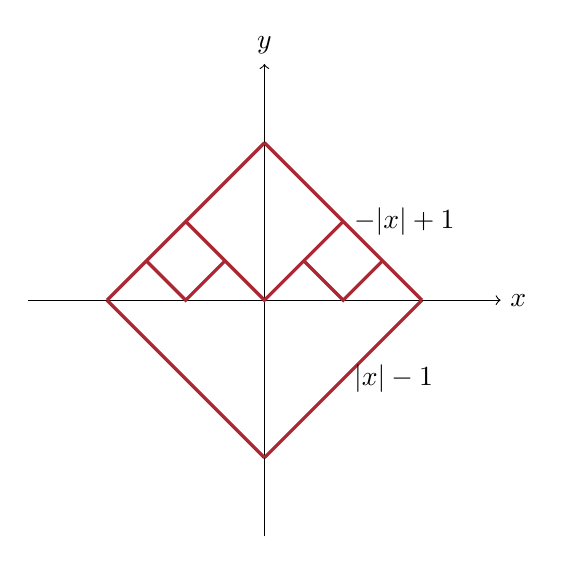
\begin{tikzpicture}[scale=2]

% Axis
      \draw[->] (-1.5,0.0) -- (1.5,0.0) node[anchor=west] {$x$};
      \draw[->] (0.0,-1.5) -- (0.0,1.5) node[anchor=south] {$y$};
% Radmacher Functions
    %k=0
      \begin{scope}[draw=Mahogany!80!Mulberry,line width=1.2pt]
        \draw (-1.0,0.0) -- (0.0,1.0);
        \draw (0.0,1.0)  -- (0.5,0.5) node[anchor=west] {$-|x|+1$} -- (1.0,0.0);

        \draw (-1.0,0.0)  -- (0.0,-1.0);
        \draw (0.0,-1.0)  -- (0.5,-0.5) node[anchor=west] {$|x|-1$} -- (1.0,0.0);
%k=1
        \draw (-0.5,0.5) -- (-0.0,0.0) -- (0.5,0.5);
%k=2
        \draw (-0.75,0.25) -- (-0.5,0.0) -- (-0.25,0.25);
        \draw (0.25,0.25) -- (0.5,0.0) -- (0.75,0.25);
      \end{scope}

    \end{tikzpicture}
  \end{center}
  \caption{Funzioni di \emph{Readmacher}. Soluzioni quasi ovunque dell'equazione einoidale.}
  \label{fig:cp2-01}
\end{figure}

Nel 1982 Crandal e Lions introdussero una differente nozione di soluzione debole (soluzioni viscose \cite[vedi][]{crand:lion}) per molte equazioni del primo e del secondo ordine, soddisfacente proprietà di esistenza, unicità e stabiltà. 
%%%%%%%%%%%%%%%%%%%%%%%%%%%%%%%%%%%%%%%%%%%%%%%%%%%%%%%%%%%%%%%%%%%%%%%%%%
%
%                            Section 2.2
%
%
%%%%%%%%%%%%%%%%%%%%%%%%%%%%%%%%%%%%%%%%%%%%%%%%%%%%%%%%%%%%%%%%%%%%%%%%%%
\section{Nozione di soluzioni viscose}
Inziamo col introdurre la definizione di soluzione viscosa per PDE del secondo ordine, cioè equazioni del tipo
\begin{equation}
\label{eq:cp2-02}
F(x,u,Du,D^2u) = 0\text{ con }F:\mathbb{R}^N\times\mathbb{R}\times\mathbb{R}^N\times S(N)\to \mathbb{R},
\end{equation}
con $S(N)$ insieme delle matrici simmetriche $N\times N$, $u$ una funzione a volori reali definita in un sottoinsieme $\mathcal{O}$ di $\mathbb{R}^N$ e $Du$,$D^2u$ corrispondono al gradiente ed alla matrice delle derivate seconde di $u$. Al fine di applicare la teoria a un equazione del tipo \eqref{eq:cp2-02} (\cite[][2]{crand:lion}), richiederemo che $F$ soddisfi le seguenti propietà
\begin{gather}
\label{eq:cp2-03}
F(x,r,p,X) \leq F(x,s,p,X) \quad \forall\,r\leq s,\\
\label{eq:cp2-04}
F(x,r,p,X) \leq F(x,r,p,Y) \quad \forall\,Y\leq X,
\end{gather}
con $r,s\in \mathbb{R},X,Y\in S(N)$ and $S(N)$ equipaggiato del solito ordine tra matrici. Se $F$ soddisfa \eqref{eq:cp2-03} allora si dirà \emph{ellitticamente degenere}, mentre se soddisfa \eqref{eq:cp2-04} si dirà \emph{propria}.

Da qui in avanti assumeremo sempre che $F$ soddisfi \eqref{eq:cp2-03}
e \eqref{eq:cp2-04} e che sia continua, a meno che non venga detto
diversamente. Prima di enunciare la definizione di soluzione di
viscosità, diamo una giustificazione euristica. Supponiamo che $u\in C^2$ su $\mathbb{R}^n$ e che
\[
F(x,u(x),Du(x),D^2u(x))\leq 0\, \forall x\in\mathbb{R}^n,
\]
cioè $u$ è una sottosoluzione classica di $F=0$. Supponiamo $\phi\in
C^2$ e $\hat{x}$ sia un massimo locale per $u-\phi$, dall'analisi
questo implica che $Du(\hat{x})=D\phi(\hat{x})$ e $D^2u(\hat{x})\leq
D^2\phi(\hat{x})$, quindi dalla \eqref{eq:cp2-03} segue
\[
F(x,u(\hat{x}),D\phi(\hat{x}),D^2\phi(\hat{x}))\leq F(x,u(x),Du(x),D^2u(x))\leq 0.
\]
Gli estremi di questa diseguaglianza non dipendono dalle derivate di $u$, quindi possiamo considerare un arbitraria funzione $u$ essere sotto soluzione di $F=0$ se
\begin{equation}
  \label{eq:cp2-01-add}
  F(x,u(\hat{x}),D\phi(\hat{x}),D^2\phi(\hat{x}))\leq 0
\end{equation}
ogniqualvolta $\phi\in C^2$ e $\hat{x}$ massimo locale di $u-\phi$.
Inoltre  per $x$ vicino a $\hat{x}$ è vero che $u(x)\leq u(\hat{x})-\phi(\hat{x}) + \phi(x)$, poichè $\phi\in C^2$ usando Taylor otteniamo
\begin{equation}
  \label{eq:cp2-05}
  u(x)\leq u(\hat{x})+\left<p,x-\hat{x}\right> + \frac{1}{2}\left<X(x-\hat{x}),x-\hat{x}\right> + o(|x-\hat{x}|^2)\,\, x\to\hat{x}
\end{equation}
con $p=D\phi(\hat{x})$ e $X=D^2\phi(\hat{x})$. Possiamo osservare che se la \eqref{eq:cp2-05} è soddisfatta per qualche $(p,X)\in\mathbb{R}^n\times S(N)$ e $u$ è due volte differenziabile, allora $p=Du(\hat{x})$ e $D^2u(\hat{x})\leq X$ (\emph{Osservazione} \ref{oss:cp2-01}). Quindi se $u$ è una soluzione classica per $F\leq 0$ segue che $F(x,u(x),p,X)\leq 0$ ogni qual volta è vera la \eqref{eq:cp2-05}. Ora possiamo dare la definizione di soluzione viscosa, che si basa proprio sulla \eqref{eq:cp2-05}
\begin{definizione}
\label{def:cp2-01}
Sia $F$ propria ed ellittica degenere e $\mathcal{O}\subset\mathbb{R}^n$.
Una sottosoluzione viscosa di $F=0$ su $\mathcal{O}$ è una funzione $u:\mathcal{O}\to\mathbb{R}$ continua tale che
\begin{equation}
  \label{eq:cp2-06}
  F(x,u(x),p,X)\leq 0\quad\forall x\in\mathcal{O}\text{ and }(p,X)\in J_{\mathcal{O}}^{2,+}u(x).
\end{equation}
Similmente, una sopra soluzione viscosa di $F=0$ su $\mathcal{O}$ è una funzione continua tale che
\begin{equation}
  \label{eq:cp2-07}
  F(x,u(x),p,X)\geq 0\quad\forall x\in\mathcal{O}\text{ and }(p,X)\in J_{\mathcal{O}}^{2,-}u(x).
\end{equation}
Infine, $u$ è una soluzione viscosa se è sia sotto che sopra soluzione.
\end{definizione}
Dove $J_{\mathcal{O}}^{2,+}u(x)$ rappresenta il \emph{superjet} del secondo ordine di $u$ nel puto $x$. Più precisamente sia $\mathcal{O}\subset\mathbb{R}^N$ arbitrario%
\footnote{Nelle dimostrazioni di esistenza, unicità e confronto viene preso localmento compatto \cite[vedi][10 §1]{crand:lion}.}
,  $u:\mathcal{O}\to\mathbb{R}$ e $\hat{x}\in\mathcal{O}$ allora
\[
J_{\mathcal{O}}^{2,+}u(\hat{x}) = \left\{(p,X)\in\mathbb{R}^n\times S(N):\,\text{ vale la \eqref{eq:cp2-05} per }\mathcal{O}\ni x\to\hat{x}\right\},
\]
quindi $J_{\mathcal{O}}^{2,+}u(x)$ definisce una mappa da $\mathcal{O}$ ad un sottoinsieme di $\mathbb{R}^n\times S(N)$. Una definizione simile si ottiene per il \emph{subjet} $J_{\mathcal{O}}^{2,-}u(x)$ basta invertire il segno della disuguaglianza.
\begin{osservazione}
Come si può notare dalla definizione, il ``superjet'' (lo stesso vale per il ``subjets'') dipende dall'insieme $\mathcal{O}$, tuttavia si può notare che il suo valore è lo stesso per tutti quegli insiemi $\mathcal{O}$ per i quali $x$ è un punto interno.  
\end{osservazione}

\begin{osservazione}
\label{oss:cp2-01}
Nella definizione di soluzione viscosa, la richiesta di continuità di $u$ può essere sostituita con quella di semicontinuà superiore(\emph{upper semicontinuos}) per le sotto soluzione e semicontinuà inferiore(\emph{lower semicontinuos}) per le sopra soluzione. Inoltre, notiamo che una funzione semicontinua sia superiormente che inferiormente è continua. Ricordiamo che  $u:L \to\mathbb{R}$ è
\begin{enumerate}
  \item \emph{upper semicontinuos} in $\hat{x}\in L$ se:
    \[
      \limsup_{x\downarrow\hat{x}}u(x)\leq u(\hat{x}).
    \]
  \item \emph{lower semicontinuos} in $\hat{x}\in L$ se:
    \[
      \liminf_{x\downarrow\hat{x}}u(x)\geq u(\hat{x}).
    \]
\end{enumerate}  

Seguendo la discussione fatta ad inizio sezione, se $u$ è una soluzione viscosa di $F\leq 0$, $\phi\in C^2$ in un intorno di $\mathcal{O}$ e $u-\phi$ ha un massimo locale in $\hat{x}\in\mathcal{O}$, allora è vera la \eqref{eq:cp2-01-add} ( stesso ragionamento per le sopra soluzioni). Questo motiva la richiesta per $u$ di essere semicontinua dall'alto (rispettivamente dal basso per le sopra soluzioni), in quanto è facile produrre massimi per funzioni semicontinue dall'alto.
Possiamo dire di più, la validità di \eqref{eq:cp2-01-add} per tutte le $\phi\in C^2$ tale che $u-\phi$ ha un massimo locale relativo ad $\mathcal{O}$, con $u$ semicontinua dall'alto, equivale a dire che $u$ è una sotto soluzione viscosa.  Infatti si può mostrare il seguente lemma (per maggiori dettagli \cite[vedi][§3]{giga:main})
\begin{lemma}
  \label{lem:cp2-01}
 Sia $\hat{x}\in\mathcal{O}$ localmente compatto%
\footnote{ Ricordiamo che un insieme di uno spazio metrico si dice localmente compatto se ogni punto ammette un intorno compatto.}
 e $u$ semicontinua dall'alto allora
\begin{enumi}
  \item  vale la seguente uguaglianza
\[
J_{\mathcal{O}}^{2,+}u(\hat{x}) = \left\{
\begin{aligned}
&(D\phi(\hat{x}),D^2\phi(\hat{x})):\\
\phi\in C^2&\text{ e $u-\phi$ ha massimo locale in $\hat{x}$}
\end{aligned}
\right\}
\]
  \item  In $(i)$ $\mathcal{O}$ può essere rimpiazzato da un intorno $\mathcal{O}'$ di $\hat{x}$ in $\mathcal{O}$.
\end{enumi}
\end{lemma}

\begin{proof}
Denotiamo con $J$ l'insieme a destra dell'uguaglianza in $(i)$ e poniamo $\hat{x}=0$ se così non fosse possiamo sempre traslare il tutto.
\begin{enumi}
\item  Prendiamo un elemento in $J$, allora $u-\phi$ ha massimo locale in $\hat{x}=0$ quindi
\[
\begin{aligned}
u(x) - u(0)\leq\phi(x) -\phi(0)&=\left<D\phi(0),x\right> + \frac{1}{2}\left<D^2\phi(0)x,x\right> +\\
+ o(|x|^2)\text{ per }x\to 0,
\end{aligned}
\]
avendo utilizzato un espansione di Taylor per $\phi$. Questo ci dice che $J_{\mathcal{O}}^{2,+}u(0)\supseteq J$.

Ora prendiamo $(p,X)\in J_{\mathcal{O}}^{2,+}u(0)$, cioè
\[
u(x) - u(0)\leq\left<p,x\right> + \frac{1}{2}\left<Xx,x\right> + \varepsilon(x),
\]
con $\varepsilon(x)/|x|^2\to 0$ per $x\to 0$.
Il problema è che $\varepsilon(x)$ non è detto che sia $C^2$. Poniamo 
\[
\omega_0(\sigma)=\sup\left\{\frac{|\varepsilon(x)|}{|x|^2}; |x|\leq\sigma,x\in\mathcal{O}\right\}
\]
così che $\omega_0$ è una funzione da $[0,\infty)$ in $[0,\infty)$ non decrescente e continua in $\sigma=0$ con $\omega_0(0)=0$, applicando un risultato noto \cite[vedi][§2 Lemma 2.1.9]{giga:main}, allora esiste una funzione $\theta\in C^2[0,\infty)$ tale che
\[
\begin{aligned}
&\omega_0(\sigma)|\sigma|^2\leq\theta(\sigma)\text{ per }\sigma\geq 0,\\
&\theta(0)=\theta'(0)=\theta''(0)=0,\,\theta'''(\sigma)\geq 0\text{ per }\sigma\geq 0.
\end{aligned}
\]
Poichè $|\varepsilon(x)|\leq\omega_0(|x|)|x|^2$, prendiamo una funzione $C^2$ del tipo
\[
\phi(x)=<p,x> + \frac{1}{2}<Xx,x> +\theta(|x|)
\]
così che $u-\phi$ ha massimo locale su $\mathcal{O}$ in $\hat{x}=0$ e $p=D\phi(0)$, $X=D^2\phi(0)$. Quindi $J_{\mathcal{O}}^{2,+}u(0)\subseteq J$.
\item  Segue dalla dimostrazione di $(i)$.
\end{enumi}
\end{proof}

\end{osservazione}

\begin{osservazione}
Si può facilmente verificare che se $u\in C^2$ è soluzione classica di \eqref{eq:cp2-02} ed $F$ è elliticamente degenere, allora $u$ è soluzione viscosa.
\end{osservazione}

\begin{esempio}
Riprendiamo l'equazione eiconale \eqref{eq:cp2-01} e mostriamo che la funzione $u(x) = -|x| + 1$ è una soluzione viscosa. Partiamo dall'osservare che questa funzione risolve classicamente l'equazione in $\mathbb{R}\setminus\{0\}$, quindi
calcoliamoci rapidamente il ``superjets'' e il ``subjets'' in $\hat{x}=0$
\[
\begin{aligned}
  J^{2,+}u(0) &= \left\{\left((-1,1)\times\mathbb{R}\right)\cup\left(\{-1,1\}\times [0,+\infty)\right)\right\}, \\
  J^{2,-}u(0) &= \left\{\emptyset\right\},
\end{aligned}
\]
applicando la definizione \ref{def:cp2-01} si osserva che $|p|\leq 1$ è vera per ogni $(p,X)\in J^{2,+}u(0)$, quindi è sotto soluzione e che $|p|\geq 1$ è banalmente verificata in quanto $J^{2,-}u(0)=\emptyset$. In conclusione $u(x)=-|x|+1$ e soluzione viscosa di \eqref{eq:cp2-01}.  
\end{esempio}

La definizione di soluzione viscosa qui presentata, può essere estesa anche al caso di equazioni paraboliche cioè del tipo
\begin{equation}
\label{eq:cp2-08}
u_t + F(t,x,u,Du,D^2u) = 0,
\end{equation}
dove ora $u=u(t,x)$ e $Du$, $D^2u$ stanno per $D_xu$ e $D^2_xu$. Per farlo dobbiamo ridefinire gli insiemi $J_{\mathcal{O}}^{2,\pm}$. Sia $\mathcal{O}\subset\mathbb{R}^N$, $T>0$ e $\mathcal{O}_T = (0,T)\times\mathcal{O}$, denotiamo con $\mathcal{P}_{\mathcal{O}}^{2,\pm}$ la variante parbolita dei ``superjets'' e ``subjets'' e andiamoli a definire; se $u:\mathcal{O}\to\mathbb{R}$ allora $\mathcal{P}_{\mathcal{O}}^{2,+}u(s,z)$ è costituito da $(a,p,X)\in\mathbb{R}\times\mathbb{R}^N\times S(N)$ se $(s,z)\in\mathcal{O}_T$ e
\[
\begin{aligned}
  u(t,x)\leq &u(s,z) +a(t-s)+\left<p,x-z\right>+\frac{1}{2}\left<X(x-z),x-z\right> \\
  &+o(|t-s|+|x-z|^2)\text{ per }\mathcal{O}_T\ni (t,x)\to(s,z),
\end{aligned}
\]
similarmente possiamo definire $\mathcal{P}_{\mathcal{O}}^{2,-}u(s,z)=-\mathcal{P}_{\mathcal{O}}^{2,+}(-u(s,z))$. Quindi in conclusione una sotto soluzione di \eqref{eq:cp2-08} su $\mathcal{O}_T$ è una funzione $u$ semicontinua dall'alto tale che
\[
a+F(t,x,u(t,x),p,X)\leq 0\text{ per }(t,x)\in\mathcal{O}_T,(a,p,X)\in\mathcal{P}_{\mathcal{O}}^{2,+}u(t,x),
\]
e una sopra soluzione una funzione semicontinua dal basso tale che
\[
a+F(t,x,u(t,x),p,X)\geq 0\text{ per }(t,x)\in\mathcal{O}_T,(a,p,X)\in\mathcal{P}_{\mathcal{O}}^{2,-}u(t,x),
\]
e quindi un soluzione viscosa se sono verificate entrambe le diseguaglianze.

\begin{osservazione}
Osserviamo che anche in questo caso $F$ soddisfa le proprietà \eqref{eq:cp2-03} e \eqref{eq:cp2-04}. Ed inoltre anche per i ``semijets'' parbolici vale un lemma del tipo \ref{lem:cp2-01} \cite[vedi][§3]{giga:main}.
\end{osservazione}

Le definizioni si posso estendere anche per $u$ ed $F$ arbitrarie, non necessariamente continue. Prima di vedere come, richiamiamo la definizione di inviluppo semicontinuo. Sia $h$ una funzione definita in $L\subset\mathbb{R}$ a valori in $\tilde{\mathbb{R}}=\mathbb{R}\cup\{\pm\infty\}$, definiamo inviluppo semicontinuo superiore $h^*$ e inferiore $h_*$ nel seguente modo
\begin{subequations}
\label{eq:cp2-03-add}
\begin{align}
  \label{eq:cp2-03-1-add}%
  h^*(x) &= \lim_{r\downarrow 0}\sup_{\substack{|x-y|<r \\ y\in L}}h(y),\quad x\in\overline{L} \uptag{*} \\
  \label{eq:cp2-03-2-add}%
  h_*(x) &= \lim_{r\downarrow 0}\inf_{\substack{|x-y|<r \\ y\in L}}h(y),\quad x\in\overline{L} \subtag{*}
\end{align}
\end{subequations}
sono rispettivamente funzioni definite sulla chiusura di $L$ a valori in $\tilde{\mathbb{R}}$. In altre parole $h_*$ è la piu grande funzione semicontinua dal basso su $\overline{L}$ che è più piccola di $h$ su $L$, mentre $h^*$ è la più piccola funzione semicontinua dall'alto in $\overline{L}$ più grande di $h$ in $L$.
Prendiamo $\mathcal{O}\subset\mathbb{R}^N$ e consideriamo un sottoinsieme denso $W$ di $\Omega(\mathcal{O})=\mathcal{O}\times\mathbb{R}\times\mathbb{R}^N\times S(N)$ e sia $F=F(x,s,p,X):W\to\mathbb{R}$. Poichè $W$ è denso in $\Omega(\mathcal{O})$, gli inviluppi semicontinui $F_*$, $F^*$ sono definiti in $\Omega(\mathcal{O})$ con valori in $\tilde{\mathbb{R}}$.
\begin{definizione}
Una funzione $u:\mathcal{O}\to\mathbb{R}$ è chiamata una sotto soluzione viscosa (rispettivamente sopra soluzione) in $\mathcal{O}$ di \eqref{eq:cp2-02} se $u^*<\infty$ (resp. $u_*>-\infty$) in $\mathcal{O}$ e per ogni coppia $\phi\in C^2(\mathcal{O})$ e $\hat{x}\in\mathcal{O}$ soddisfacente $\max_{\mathcal{O}}(u^*-\phi)=(u^*-\phi)(\hat{x})$ (resp. $\min_{\mathcal{O}}(u_*-\phi)=(u_*-\phi)(\hat{x})$), vale che
\[
\begin{aligned}
&F_*(\hat{x},u^*(\hat{x}),D\phi(\hat{x}),D^2\phi(\hat{x}))\leq 0 \\
(\text{resp. }&F^*(\hat{x},u_*(\hat{x}),D\phi(\hat{x}),D^2\phi(\hat{x}))\geq 0)
\end{aligned}
\]
\end{definizione}
\begin{osservazione}
Applicando il lemma \ref{lem:cp2-01} possiamo dara una definizione generica di soluzione viscosa per l'equazione \eqref{eq:cp2-02} utilizzando i ``superjets'' e ``subjets''.
\end{osservazione}
Una definizione generica analoga vale anche nel caso di equazioni paraboliche del tipo \eqref{eq:cp2-08}.
\begin{definizione}
\label{def:cp2-02}
Una funzione $u:\mathcal{O}_T\to\mathbb{R}$ è chiamata una sotto soluzione viscosa (rispettivamente sopra soluzione) in $\mathcal{O}_T$ di \eqref{eq:cp2-08} se $u^*<\infty$ (resp. $u_*>-\infty$) in $\mathcal{O}_T$ e per ogni coppia $\phi\in C^2(\mathcal{O}_T)$ e $(\hat{x},\hat{t})\in\mathcal{O}_T$ soddisfacente $\max_{\mathcal{O}_T}(u^*-\phi)=(u^*-\phi)(\hat{x},\hat{t})$ (resp. $\min_{\mathcal{O}_T}(u_*-\phi)=(u_*-\phi)(\hat{x},\hat{t})$), vale che
\[
\begin{aligned}
&\phi_t(\hat{x},\hat{t}) + F_*(\hat{x},\hat{t},u^*(\hat{x},\hat{t}),D\phi(\hat{x},\hat{t}),D^2\phi(\hat{x},\hat{t}))\leq 0 \\
(\text{resp. }&\phi_t(\hat{x},\hat{t})+F^*(\hat{x},\hat{t},u_*(\hat{x},\hat{t}),D\phi(\hat{x},\hat{t}),D^2\phi(\hat{x},\hat{t}))\geq 0)
\end{aligned}
\]
\end{definizione}
\begin{osservazione}
In questo caso chiaramente $F$ è definita in $W_T$ denso in $\mathcal{O}_T\times\mathbb{R}\times\mathbb{R}^N\times S(N)$. E anche in questo caso possiamo dara una definizione che coinvolge i ``superjets'' e ``subjets'' parabolici, grazie ad una variante del lemma \ref{lem:cp2-01}. 
\end{osservazione}
Per risultati di esistenza, unicità e confronto sia per equazioni del tipo \eqref{eq:cp2-02} che \eqref{eq:cp2-08} \cite[vedi][]{crand:lion,giga:main,yun:giga}.
%%%%%%%%%%%%%%%%%%%%%%%%%%%%%%%%%%%%%%%%%%%%%%%%%%%%%%%%%%%%%%%%%%%%%%%%%%
%
%                            Section 2.3
%
%
%%%%%%%%%%%%%%%%%%%%%%%%%%%%%%%%%%%%%%%%%%%%%%%%%%%%%%%%%%%%%%%%%%%%%%%%%%
\section{Soluzioni viscose per il moto per curvatura media}
In questa sezione tratteremo equazioni paraboliche degeneri (cioè che verificano \eqref{eq:cp2-04}) del tipo
\begin{equation}
  \label{eq:cp2-09}
u_t + F(x,t,Du,D^2u) = 0
\end{equation}
in particolare nel caso in cui \eqref{eq:cp2-09} rappresenta un'equazione di evoluzione per superfici di livello di $u$.  Supporremo che $F$ sia geometrica cioè
\begin{equation}
  \label{eq:cp2-10}
F(x,t,\lambda p,\lambda X + \sigma p\otimes p) = \lambda F(x,t,p,X),\quad\lambda>0,\,\sigma\in\mathbb{R},
\end{equation}
per $p\in\mathbb{R}^N$ diverso da zero, $X\in S(N)$ e $\otimes$ denota il prodotto tensoriale in $\mathbb{R}^N$. Un tipico esempio di equazione che rientra in questo caso è
\[
u_t - |Du|\Div(\frac{Du}{|Du|}) = 0,
\]
l'equazione del moto per curvatura media. Iniziamo col vedere, tramite semplici conti, che questa verifica la condizione geometrica e di degenere ellitticità.
Come vedremo in dettaglio nella sezione successiva l'equazione per curvatura media si può riscrivere nel seguente modo
\[
u_t+F(Du,D^2u)=0,\quad\text{ con }F(p,X) = -\trace\left(\left(I-\frac{p}{|p|}\otimes\frac{p}{|p|}\right)X\right),
\]
con $I$ matrice identità $N\times N$.
Un semplice calcolo mostra che
\[
\begin{aligned}
F(\lambda p,\lambda X +\sigma p\otimes p)&=-\trace\left(\left(I-\frac{p}{|p|}\otimes\frac{p}{|p|}\right)\left(\lambda X+\sigma p\otimes p\right)\right)=\\
&=\lambda F(p,X)-\sigma\trace\left(\left(I-\frac{p}{|p|}\otimes\frac{p}{|p|}\right)p\otimes p\right).
\end{aligned}
\]
Poichè $(\overline{p}\otimes\overline{p})(p\otimes p)=p\otimes p$, con $\overline{p}=p/|p|$, la \eqref{eq:cp2-10} è banalmente verificata. Per dimostrare la condizione di degenere ellitticità basta mostrare che
\[
-\trace\left(\left(I-\frac{p}{|p|}\otimes\frac{p}{|p|}\right)\left(X-Y\right)\right)\leq 0\text{ con }X\geq Y.
\]
Osserviamo che la traccia del prodotto di due matrici definite non
negative è non negativo e poichè $X-Y\geq 0$,  basta mostrare che la matrice $B(p)= I-\overline{p}\otimes\overline{p}$, con $\overline{p}$ come sopra, è non negativa per $p\ne 0$, cioè che $\forall x\in\mathbb{R}^N$ $x^tB(p)x\geq 0$:
\[
x^tB(p)x=x^tx-x^t\frac{p}{|p|}\otimes\frac{p}{|p|}x=|x^2|-\frac{|p^tx|^2}{|p|^2}\geq |x|^2-\frac{|p|^2}{|x|^2}{|p|^2}=0
\]
nel penultimo passaggio abbiamo usato la disuguaglianza di Cauchy-Schwartz.

Risultati di esistenza, unicità e confronto sono stati dimostrati  per \eqref{eq:cp2-09} con
\begin{equation}
\label{eq:cp2-02-add}
u(0,x)=a(x)\in C_{\alpha}(\mathbb{R}),
\end{equation}
cioè $a(x)-\alpha$ è continua con supporto compatto in $\mathbb{R}^N$
ed $\alpha\in\mathbb{R}$ e per $F(x,t,p$\\$,X)$ ellitticamente degenere, geometrica, continua in $\mathbb{R}^N\times(0,T]\times(\mathbb{R}^N\setminus\{0\})\times S(N)$ e soddisfacente ulteriori due proprietà
\begin{subequations}
  \label{eq:cp2-12}
  \begin{align}  \label{eq:cp2-12-1}
    F_*(x,t,p,-I)&\leq c_{-}(|p|), \subtag{-}\\
     \label{eq:cp2-12-2} F^*(x,t,p,I)&\geq -c_{+}(|p|),  \subtag{+}
  \end{align}
\end{subequations}
per qualche $c_{\pm}(\sigma)\in C^1[0,\infty)$ e $c_{\pm}(\sigma)\geq c_0>0$ per qualche costante $c_0$. Iniziamo col notare che la $F$ del moto per curvatura media soddisfa le condizioni (\hyperref[eq:cp2-12-1]{\ref{eq:cp2-12}\ped{$\pm$}}); difatti $F(p,X)=-\trace\left(A(p)X\right)$ ed  essendo $F$ continua per $p\in\mathbb{R}^N\setminus\{0\}$ e geometrica  verifica le condizioni precedenti con
\[
c_{\pm}(\sigma)=\sup_{|p|=1}\trace\left(A(p)\right).
\]  
Per $p\ne 0$ abbiamo
\[
F_*(p,-I)=F(p,-I)=\trace\left(A(\overline{p})I\right)\leq\sup_{\overline{p}}\trace\left(A(\overline{p})\right)\text{ con }\overline{p}=p/|p|
\]
mentre per $p=0$, usando la definizione di inviluppo semicontinuo, otteniamo
\[
F_*(0,-I)=\inf_{|\overline{q}|=1}\trace\left(A(\overline{q})I\right)\leq\sup_{|\overline{q}|=1}\trace\left(A(\overline{q})\right),
\]
quindi soddisfa la \eqref{eq:cp2-12-1}; similmente si dimostra la \eqref{eq:cp2-12-2}.
\begin{osservazione}
Sotto le condizioni (\hyperref[eq:cp2-12-1]{\ref{eq:cp2-12}\ped{$\pm$}}), possiamo costruirci una sotto e sopra soluzione dell'equazione per il moto per curvatura media, per farlo basta applicare il seguente lemma
\begin{lemma}
Supponiamo $F$ geometrica e soddisfacente (\hyperref[eq:cp2-12-1]{\ref{eq:cp2-12}\ped{$\pm$}}) per qualche $c_{\pm}(\sigma)\in C^1[0,\infty)$ e $c_{\pm}(\sigma)\geq c_0>0$ per qualche costante $c_0$. Poniamo \[
u^{\pm}=\pm(t+\omega_{\pm}(\rho)),\quad \rho=|x|,\quad\omega_{\pm}(\rho)=\int_0^{\rho}\frac{\sigma}{c_{\pm}(\sigma)}d\sigma.
\]
Allora $u^-$ (resp. $u^+$) è una  sotto soluzione $C^2$ di \eqref{eq:cp2-09} in $\mathbb{R}\times\mathbb{R}^N$.
\end{lemma}
\begin{proof}
Dimostriamo il caso in cui $u^-$ è sotto soluzione se verifica la \eqref{eq:cp2-12-1}, l'altro è analogo. Per definizione di $u^-\in C^2(\mathbb{R}\times\mathbb{R}^N)$. Poichè $F_*$ è geometrica e
\[
\begin{aligned}
D&\omega_{-}(\rho)=\omega_{-}^{'}(\rho)D\rho \\
D^2\omega_{-}(\rho)&=\omega_{-}^{''}(\rho)D\rho\otimes D\rho+\omega_{-}^{'}(\rho)D^2\rho \\
&D^2\rho = \rho^{-1}(I-D\rho\otimes D\rho)
\end{aligned}
\]
dove l'ultima uguaglianza deriva dal fatto che $D\rho = D|x| = x/\rho$, quindi derivando giungiamo al risultato riportato sopra. Osservando che $\omega_{-}^{'}(\rho)> 0$ un semplice calcolo ci mostra che
\[
\begin{aligned}
F_*(x,t,Du,D^2u) &= F_{*}(x,t,-\omega_{-}^{'}(\rho)D\rho,-\omega_{-}^{'}(\rho)\rho^{-1}I+\sigma D\rho\otimes D\rho) \\
&=\omega_{-}^{'}(\rho)\rho^{-1}F_*(x,t,-\rho D\rho,-I),
\end{aligned}
\] 
con $\sigma = -(\omega^{''}(\rho)-\omega^{'}(\rho))$.
In conclusione abbiamo
\[
u_t + F_*(x,t,Du,D^2u) = -1 + \frac{1}{c_{-}(\rho)}F_*(x,t,-x,-I),
\]
in quanto  $\rho D\rho=x$, quindi per la \eqref{eq:cp2-12-1} otteniamo
\[
u_t + F_*(x,t,Du,D^2u)\leq 0
\]
e per la definizione \ref{def:cp2-02}, $u$ è sotto soluzione viscosa di \eqref{eq:cp2-09}.
\end{proof}
Applicando tale lemma con $c_{\pm}(\sigma)=\sup_{|\overline{p}|=1}\trace\left(A(\overline{p})\right)=N-1$ con $A(\overline{p})=I-\overline{p}\otimes\overline{p}$ otteniamo che
\[
u^{-}=-\left(t+\frac{|x|^2}{2(N-1)}\right).
\]
è una soluzione viscosa del moto per curvatura media, che rappresenta sfere che si contraggono. 
\end{osservazione}
Nel lavoro di Giga, Chen e Goto sono stati dimostrati teoremi di
esistenza, confronto e unicità per \eqref{eq:cp2-09} e dato iniziale
\eqref{eq:cp2-02-add}, noi qui riportiamo solo l'enunciato del
teoremi esistenza; per approfondimenti e dimostrazioni si veda \cite[][§4-6]{yun:giga}.
\begin{teorema}[Esistenza globale]
Sia $T>0$. Assumiamo che $F(t,p,X)$ sia continua in $(0,T]\times(\mathbb{R}^N\setminus\{0\})\times S(N)$, geometrica, ellitica degenere, soddisfacente le condizioni (\hyperref[eq:cp2-12-1]{\ref{eq:cp2-12}\ped{$\pm$}}) e tale che $ -\infty<F_*(t,0,O) = F^*(t,0,O)<\infty$, con  $O$ matrice $N\times N$ nulla. Allora per $a\in C_{\alpha}(\mathbb{R}^N)$ esiste una unica soluzione viscosa $u_a\in C_{\alpha}([0,T]\times\mathbb{R}^N)$ di \eqref{eq:cp2-09}-\eqref{eq:cp2-02-add} 
\end{teorema}
Per completare questa sezione, e per definire le soluzioni nel caso particolare del moto per curvatura media, vediamo come definire 
\[
F(p,X)=-\trace\left(\left(I-\overline{p}\otimes\overline{p}\right)X\right)
\]
in $p=0$, punto in cui è discontinua. In questo scenario c'è abbastanza arbitrarietà nello scegliere il valore di $F$, questo perchè come osservato da Crandal e Lions nell'analisi dell'equazione andiamo a porre $X=0$ quando $p=0$, quindi il valore in $p=0$ non importa purchè sia consistente  \cite[vedi][§9 p53]{crand:lion}.
\begin{enumi}
  \item Una prima possibilità è quella di calcolare esplicitamente gli inviluppi semicontinui $F_*$ e $F^*$ usando le definizione \eqref{eq:cp2-03-1-add} e \eqref{eq:cp2-03-2-add}, facciamo il conto per $F_*$
\[
F_*(0,X)=\lim_{r\downarrow 0}\inf_{\substack{|q|<r \\ q\in \mathbb{R}^N\setminus\{0\}}}F(q,X),
\]
ora $F(q,X)=-\trace\left(X\right)+\trace\left(\left(\overline{q}\otimes\overline{q}\right)X\right)$, con $\overline{q}=q/|q|$, quindi
\[
F_*(0,X)=-\trace\left(X\right)+\inf_{\substack{|\overline{q}|=1 \\ \overline{q}\in \mathbb{R}^N\setminus\{0\}}}\trace\left(\left(\overline{q}\otimes\overline{q}\right)X\right).
\]
Calcoliamoci il secondo addento dell'equazione precedente. Per farlo
ricordiamo che una matrice simmetrica a valori reali, come è $X$, è
diagonalizzabile con matrici ortonormali (Teorema spettrale) quindi
esiste $U$ tale che $UU^t=I$ e $X=U^t\Lambda U$, dove
$\Lambda=diag(\lambda_i(X))$, per ${\{i=1\dots n\}}$, con $\lambda_i$ autovalori di $X$. Applicando una propietà della traccia, ossia $\trace(AB)=\trace(BA)$, otteniamo che 
\[
\trace\left((\overline{q}\otimes\overline{q})X\right)=\trace\left((\overline{q}\otimes\overline{q})\Lambda\right)
\]
quindi
\[
\inf_{\substack{|\overline{q}|=1 \\ \overline{q}\in \mathbb{R}^N\setminus\{0\}}}\trace\left(\left(\overline{q}\otimes\overline{q}\right)X\right) = \inf_{\substack{|\overline{q}|=1 \\ \overline{q}\in \mathbb{R}^N\setminus\{0\}}}\sum_{i=1}^nq_i^2\lambda_i(X)
\]
con $q_i$ componenti del vettore $\overline{q}$. Il termine a destra dell'uguaglianza precednte è pari a $\lambda_{\text{min}}(X)$, mentre se ripetiamo il calcolo per $F^*$ nell'espressione precedente otterremo un $\sup\sum_{i=1}^nq_i^2\lambda_i(X)$ che è pari a $\lambda_{\text{max}}(X)$ (vedi \emph{osservazione} \ref{oss:cp2-02}).
Quindi $F^*$ e $F_*$ da usare nella definizione \ref{def:cp2-02} di soluzioni viscose per l'equazione del moto per curvatura media, sono
\begin{subequations}
\begin{align}
  \label{eq:cp2-13-1}%
  F_*(p,X) &=%
  \begin{cases}
   -\trace\left(\left(I-\overline{p}\otimes\overline{p}\right)X\right) &\text{ se } p\ne 0 \\
   -\trace\left(X\right)+\lambda_{\text{min}}(X) & \text{ se }p = 0
  \end{cases} \subtag{lse}\\
  \label{eq:cp2-13-2}%
  F^*(p,X) &=%
  \begin{cases}
   -\trace\left(\left(I-\overline{p}\otimes\overline{p}\right)X\right) &\text{ se } p\ne 0 \\
   -\trace\left(X\right)+\lambda_{\text{max}}(X) & \text{ se }p = 0
  \end{cases} \subtag{use}
\end{align}
\end{subequations}
\begin{osservazione}
  \label{oss:cp2-02}
  Proviamo che 
\[
\lambda_{\text{min}}(X)\leq\sum_{i=1}^nq_i^2\lambda_i(X)\leq\lambda_{\text{max}}(X),\quad |q| = 1,
\]
per induzione su $n$.
\begin{itemize}
  \item $N=1$, ovvia niente da dimostrare
  \item $N=2$, otteniamo che
\[
\sum_{i=1}^2q_i^2\lambda_i=\lambda_{\text{min}} + q_{\text{max}}^2(\lambda_{\text{max}}-\lambda_{\text{min}}),
\]
quindi essendo $q_{\text{max}}^2\leq 1$ il valore della somma precedente è sempre compresa tra il minimo ed il massimo dei valori $\lambda_{1,2}$ che ricordiamo essere numeri reali.
  \item $N=n$, supponiamo per semplicità che $\lambda_{\text{min}}=\lambda_1$
\[
\sum_{i=1}^nq_i^2\lambda_i=\lambda_1+\sum_{i=1}^{n-1}\hat{q}_i^2\hat{\lambda}_i,
\]
con $\hat{\lambda}_i=(\lambda_i-\lambda_1)>0$ e $\hat{q}=(q_2,\dots,q_n)$, $|\hat{q}|\leq 1$. Ora supponiamo, sempre per semplicità, $\hat{\lambda}_1$ il minimo dei $\hat{\lambda}_i$ e applicando l'ipotesi induttiva abbiamo
\begin{align}
0\leq\sum_{i=1}^{n-1}\hat{q}_i^2\hat{\lambda}_i(X)&=\hat{\lambda}_1|\hat{q}|+\sum_{i=2}^{n-1}\hat{q}_i^2(\hat{\lambda}_i-\hat{\lambda}_1) \notag\\
\hat{\lambda}_1|\hat{q}|+\sum_{i=2}^{n-1}\hat{q}_i^2(\hat{\lambda}_i-\hat{\lambda}_1)&\leq \hat{\lambda}_1+\sum_{i=2}^{n-1}\hat{q}_i^2(\hat{\lambda}_i-\hat{\lambda}_1)\leq\hat{\lambda}_{\text{max}}\notag \\
\intertext{e quindi}
\lambda_1=\lambda_{\text{min}}&\leq\sum_{i=1}^nq_i^2\lambda_i\leq\lambda_{\text{max}}\notag
\end{align}

\end{itemize}
\end{osservazione}
  \item Una altra definizione è quella proposta da Crandal e Lions \cite[vedi][§9]{crand:lion}
\begin{subequations}
\label{eq:cp2-14}
\begin{align}
  \label{eq:cp2-14-1}%
  \underline{F}(p,X) &=%
  \begin{cases}
   -\trace\left(\left(I-\overline{p}\otimes\overline{p}\right)X\right) &\text{ se } p\ne 0 \\
   -2||X|| & \text{ se }p = 0
  \end{cases} \subtag{cl_*}\\
  \label{eq:cp2-14-2}%
  \overline{F}(p,X) &=%
  \begin{cases}
   -\trace\left(\left(I-\overline{p}\otimes\overline{p}\right)X\right) &\text{ se } p\ne 0 \\
   +2||X|| & \text{ se }p = 0
  \end{cases} \subtag{cl^*}
\end{align}
\end{subequations}
Queste  sono  \eqref{eq:cp2-14-1} semicontinua inferiormente e
\eqref{eq:cp2-14-2} superiormente per $n=2,3$, \cite[vedi][§9]{crand:lion}.
\end{enumi}
\begin{osservazione}
Osserviamo che i teoremi sopra esposti valgono nel caso di moto per curvaura media, come abbiamo mostrato,  ed anche per la sua  generalizzazione cioè
\[
u_t -|Du|\Div\left(\frac{Du}{|Du|}\right) - \nu|Du| = 0,\quad\nu\in\mathbb{R},
\]
il cui flusso continua a verificare le ipotesi del teorema.
 Tuttavia possiamo estendere risultati di confronto ed esistenza, anche nel caso dell'equazione del moto per curvatura media che preserva il volume
\begin{equation}
  \label{eq:cp2-15}
  u_t(x,t)=|Du(x,t)|\Div{\left(\frac{Du(x,t)}{|Du(x,t)|}\right)}-\frac{\iint\Div{\left(\frac{Du(x,t)}{|Du(x,t)|}\right)}d\mu}{3V_0}x^tDu
\end{equation}
Sia $u:\Omega\times(0,T)\to\mathbb{R}$, una funzione level set di qualche superficie, allora l'integrale dell'equazione precedente lo possiamo riscrivere (vedi §\ref{sec:cp3-sc3-3})
\[
\mathcal{I}(u(x,t),t)=\frac{\int_{\Omega}-F(Du,D^2u)\delta(u(x,t))dx}{3V_0},
\]
Se tale termine ha una dipendenza locale da $u$ (come nel caso della
sfera in cui risulta essere costante vedi §\ref{sec:cp3-sc3-3}) allora la \eqref{eq:cp2-15} diventa
\[
u_t + F(Du,D^2u) + f(t,x,Du) = u_t +\tilde{F}(x,t,Du,D^2u)=0,
\]
con $F$ la stessa del moto per curvatura media e $f(x,t,Du)=\mathcal{I}(t)<x,Du>$.
Possiamo osservare che il flusso precedente rientra in 
\begin{equation}
\label{eq:cp2-16}
F(x,t,r,p,X) = F_0(t,r,p,X)+F_1(x,t,p),
\end{equation}
con $F_0$ soddisfacente le seguenti proprietà
\begin{enump}{f}
  \item $F_0:\overline{\Omega}\times[0,T]\times\mathbb{R}\times(\mathbb{R}^N\setminus{0})\times S(N)\to\mathbb{R}$ è continua
  \item $F_0$ ellittica degenere, cioè verifica la \eqref{eq:cp2-04}
  \item $ -\infty<F_*(x,t,0,O) = F^*(x,t,0,O)<\infty$
  \item Per qualche costante $c_0$ 
\[
      r\to F(x,t,r,p,X)+c_0r
\]
è una funzione non decrescente
\end{enump}
ed $F_1\in C(\overline{\Omega}\times[0,T]\times\mathbb{R}^N)$ tale che
\[
|F_1(x,t,p)-F_1(y,t,p)|\leq C(1+|p|)|x-y|,
\]
con qualche costante $C>0$ indipendente da $x$,
$y\in\overline{\Omega}$ e $p\in\mathbb{R}^N$. Sotto queste ipotesi,
risultati di confronto e esistenza vengono raggiunti da Crandal e
Lions, Giga e Goto, nel caso $\Omega$ limitato, per approfondimenti,
teoremi e dimostrazioni \cite[vedi][§3]{giga:main} e
\cite[][§8]{crand:lion}.
Nel caso di dipendenza non locale da $u$ in $\mathcal{I}(u,t)$, la
questione è ancora aperta e finora non sono stati raggiunti
risultati definitivi.
\end{osservazione}




\chapter{Costruzione ed analisi dello schema Semi-Lagrangiano}
\label{cp:cp2-00}
In questo capitolo costruiremo ed analizzeremo uno schema Semi-Lagrangiano per l'equazione di curvatura media in $\mathbb{R}^3$.
Ricordiamo la nostra equazione :
\begin{equation}
\label{eq:cp3-01}
\begin{cases}
u_t = \Div\left(\frac{Du}{|Du|}\right)|Du|\quad (x_1,x_2,x_3)\in\mathbb{R}^3,t\in(0,T) \\
u(x,0) = u_0(x) \qquad \quad \mathbb{R}^3\times\{t = 0\}
\end{cases}
\end{equation}
con $Du$ il gradiente di $u$.
%%%%%%%%%%%%%%%%%%%%%%%%%%%%%%%%%%%%%%%%%%%%%%%%%%%%%%%%%%%%%%%%%%%%%%%%%%%%%
% Section 3.1 Costruzione dello schema
%
%%%%%%%%%%%%%%%%%%%%%%%%%%%%%%%%%%%%%%%%%%%%%%%%%%%%%%%%%%%%%%%%%%%%%%%%%%%%%%%%
\section{Costruzione dello schema MCM}

Partiamo dall'equazione \eqref{eq:cp3-01} e operiamo alcune manipolazioni algebriche, al fine di scrivere diversamente il termine del flusso. 
\begin{proposizione}
Vale la seguente serie di uguaglianze:
\[
\Div\left(\frac{Du}{|Du|}\right)|Du|=\trace\left(\left(I-\frac{DuDu^t}{|Du|^2}\right)D^2u\right)=\vec{v}_1^tD^2u\vec{v}_1+\vec{v}_2^tD^2u\vec{v}_2.
\]
con $\vec{v}_1$ e $\vec{v}_2$ autovettori della matrice $P=I-\frac{DuDu^t}{|Du|^2}$, definiti da :
\[
\vec{v_1}=
\begin{bmatrix}
\frac{-u_{x_3}}{\sqrt{u_{x_1}^2+u_{x_3}^2}} \\
0 \\
\frac{u_{x_1}}{\sqrt{u_{x_1}^2+u_{x_3}^2}}
\end{bmatrix}
\quad
\vec{v_2}=\frac{1}{|Du|}
\begin{bmatrix}
\frac{-u_{x_1}u_{x_2}}{\sqrt{u_{x_1}^2+u_{x_3}^2}} \\
\sqrt{u_{x_1}^2+u_{x_3}^2} \\
\frac{-u_{x_2}u_{x_3}}{\sqrt{u_{x_1}^2+u_{x_3}^2}}
\end{bmatrix}
\]
\end{proposizione}
\begin{proof}
Iniziamo con la prima uguaglianza, svolgendo esplicitamente $\Div\left(\frac{Du}{|Du|}\right)$ (senza riportare tutti i conti) otteniamo :
\[
|Du|\Div\left(\frac{Du}{|Du|}\right)=|Du|\left(\frac{\Div(Du)}{|Du|} -(Du)^tD^2u\frac{Du}{|Du|^3}\right) =
\]
\[
= \Delta u - \left<D^2u\frac{Du}{|Du|},\frac{Du}{|Du|}\right> .
\]
Ora ricordando che $\Delta u$ rappresenta il laplaciano della funzione $u$ e osservando che :
\[
\left<D^2u\frac{Du}{|Du|},\frac{Du}{|Du|}\right> = \left<\frac{1}{|Du|}(u_{x_1}(D^2u)^1+u_{x_2}(D^2u)^2+u_{x_3}(D^2u)^3),\frac{Du}{|Du|}\right> =
\]
\[
=\frac{1}{|Du|^2}(u_{x_1}<(D^2u)^1,Du>+u_{x_2}<(D^2u)^2,Du>+u_{x_3}<(D^2u)^3,Du> = 
\]
\[
=\trace\left(\frac{DuDu^t}{|Du|^2}D^2u\right),
\]
avendo indicato con $(D^2u)^n$ l'$n$-esima colonna della matrice delle derivate seconde della funzione $u$, giungiamo all'uguaglianza cercata:
\[
\Div\left(\frac{Du}{|Du|}\right)|Du| = \trace\left(\left(I-{\frac{DuDu^t}{|Du|^2}}\right)D^2u\right).
\] 
Ora occupiamoni della seconda uguaglianza. Iniziamo con il fare alcune osservazioni sulla matrice $P=I-\frac{DuDu^t}{|Du|^2}$. Questa è una matrice di proiezione, $3\times3$ a valori in $\mathbb{R}$, simmetrica ($P^t=P$) e idempotente ($P^2=P$), ammette due autovettori $\vec{v}_1$,$\vec{v}_2$ e vale la seguente decomposizione
\[
P=\sum_{i=1}^2\vec{v}_i\vec{v}_i^t=\sigma\sigma^t\quad\text{ con } \sigma=[\vec{v_1},\vec{v_2}],
\]
con $\sigma$ matrice $3\times2$ che ha come colonne gli autovettori di $P$. Detto ciò abbiamo: 
\[
\trace\left(\left(I-{\frac{DuDu^t}{|Du|^2}}\right)D^2u\right)=\trace\left(\sigma\sigma^tD^2\right)=\trace\left([\vec{v}_1,\vec{v}_2][\vec{v}_1,\vec{v}_2]^tD^2u\right)=
\]
\[
=\trace\left((\vec{v}_1\vec{v}_1^t+\vec{v}_2\vec{v}_2^t)D^2u\right)=\trace\left(\vec{v}_1\vec{v}_1^tD^2u\right)+\trace\left(\vec{v}_2\vec{v}_2^tD^2u\right)
\]
Ricordando i calcoli fatti nella dimostrazione della prima uguaglianza possiamo scrivere:
\[
\begin{split}
&\trace\left(\vec{v}_1\vec{v}_1^tD^2u\right)+\trace\left(\vec{v}_2\vec{v}_2^tD^2u\right)=\left<D^2u\vec{v}_1,\vec{v}_1\right>+\left<D^2u\vec{v}_2,\vec{v}_2\right>=\\
& =\vec{v}_1^tD^2u\vec{v}_1+\vec{v}_2^tD^2u\vec{v}_2.
\end{split}
\]
\end{proof}

Riformuliamo l'equazione \eqref{eq:cp3-01} nel seguente modo :
\begin{equation}
u_t=\vec{v}_1^tD^2u\vec{v}_1 + \vec{v}_2^tD^2u\vec{v}_2,
\end{equation}
e costruiamoci il metodo.
Approssimiano la derivata temporale con le differenze finite in avanti, mentre per il termine del flusso utilizziamo le derivate direzionali scegliendo come incremento $\sqrt{2\Delta t}$.
Quindi nel caso in cui $Du \ne 0$ e $u_{x_1}^2+u_{x_3}^2\ne 0$ otteniamo :
\[
\begin{split}
&\frac{u(x,t+\Delta t)-u(x,t)}{\Delta t} +O(\Delta t)= \frac{1}{4\Delta t}\bigl[u(x+\sqrt{2\Delta t}(\vec{v}_1+\vec{v}_2),t) +\\
& +u(x+\sqrt{2\Delta t}(-\vec{v}_1+\vec{v}_2),t) + u(x+\sqrt{2\Delta t}(\vec{v}_1-\vec{v}_2),t) \\
& + u(x+\sqrt{2\Delta t}(-\vec{v}_1-\vec{v}_2),t) - 4u(x,t)\bigr] + O(\Delta t)
\end{split}
\]
Osservando tale approssimazione, possiamo notare che i punti $(x + \sqrt{2\Delta t}(\pm\vec{v}_1 \pm\vec{v}_2))$ non necessariamente saranno i nodi della griglia, quindi è necessario introdurre un operatore di interpolazione $I[\cdot]$.
Per completare la costruzione consideriamo una griglia spaziale $x_j=(j_1\Delta x,j_2\Delta x,j_3\Delta x)$ con $j=(j_1,j_2,j_3)$ multi-indice in $\mathbb{Z}^3$ ed una griglia temporale $t^n=n\Delta t$ con $n\in\mathbb{N}$.
Indichiamo con $u_j^n$ l'approssimazione di $u$ nel punto della griglia $(x_j,t^n)$ e con $D_j^n$ l'approssimazione del gradiente di $u$ nel suddetto punto. Quindi il nostro schema semi-lagrangiano risulta :
\begin{equation}
\label{eq:cp3-02}
u_j^{n+1} = \frac{1}{4}\sum_{+,-}I[u^n](x_j+\sqrt{2\Delta t}(\pm\vec{v}_1\pm\vec{v}_2)).
\end{equation} 
\begin{osservazione}
Questa costruzione non è applicabile nel caso in cui 
\begin{equation}
\label{eq:cp3-01-add}
Du = 0 \text{ o } u_{x_1}^2+u_{x_3}^2 = 0. 
\end{equation}
Quindi per distinguere i due casi dal punto di vista numerico, introduciamo una soglia $s$ ed una costante $C$. In modo tale che il verificarsi del caso \eqref{eq:cp3-01-add} è rappresentato numericamente dalle disequazioni
\[
|D_j^n|\le C\Delta x^s\text{ e }|(D_j^n)_1^2+(D_j^n)_3^2|\le C\Delta x^s.
\]
\end{osservazione}
Nel caso in cui siamo sotto la soglia, possiamo procedere in due modi diversi.
\begin{enumerate}
  \item Approssimiamo la nostra soluzione nel punto $(x_j,t^{n+1})$, con la media dei primi vicini:
    \begin{equation}
      \label{eq:cp3-03-add}
      u_j^{n+1}=\frac{1}{6}\sum_{i\in\delta(j)}u_i^n,
    \end{equation}
dove $\delta(j)=\left\{(j_1\pm 1,j_2,j_3),(j_1,j_2\pm 1,j_3),(j_1,j_2,j_3\pm 1)\right\}$. Questa rappresentazione, non è altro che un'approssimazione dell'equazione del calore $u_t=\varepsilon\Delta u$ in $\mathbb{R}^3\times(0,T)$. Difatti usando Eulero in avanti per la derivata temporale e differenze finite centrate per quella spaziale abbiamo:
\[
\begin{aligned}
  \frac{u_j^{n+1}-u_j^n}{\Delta t}=\varepsilon&\frac{u_{j_1 + 1,j_2,j_3}^n +
    u_{j_1 - 1,j_2,j_3}^n + u_{j_1,j_2 + 1,j_3}^n + u_{j_1,j_2 - 1,j_3}^n}{\Delta x^2} + \\
    &+ \frac{u_{j_1,j_2,j_3 + 1}^n + u_{j_1,j_2,j_3 - 1}^n - 6u_j^n}{\Delta x^2},
\end{aligned}
\]
scegliendo $\varepsilon=\frac{\Delta x^2}{6\Delta t}$ otteniamo la \eqref{eq:cp3-03-add}.
Tale scelta è giustificata dal fatto che, come vedremo nella sezione successiva, il moto per curvature media è consistente con l'approssimazione dell'equazione del calore a patto di adottare, come soluzione viscosa, la definizione (riferimento formula) proposta da \emph{Crandall} \cite[vedi][]{crand:lion}.

  \item Utilizziamo l'approssimazione dell'equazione $u_t=\frac{1}{2}\Delta u$:
    \begin{equation}
      \label{eq:cp-04-add}
      u_j^{n+1}=u_j^n +\frac{1}{2}\frac{\Delta t}{\Delta x^2}\left(6u_j^n - \sum_{i\in\delta(j)}u_i^n\right).
    \end{equation}
Tale scelta è giustificata, in quanto il moto per curvatura media risulta essere consistente con l'equazione $u_t=\frac{1}{2}\Delta u$, (vedi sezione successiva) prendendo come soluzione viscosa la definizione standard (riferimento formula) \cite[vedi][]{fed:drag}. L'unico problema è che la \eqref{eq:cp-04-add}
richiede una $\mathit{CFL}$ parabolica, che non è presente nel nostro schema essendo \emph{semi-lagrangiano}; un modo per aggirare il problema è quello di usare uno schema implicito nell'approssimazione di  $u_t=\frac{1}{2}\Delta u$.
\end{enumerate}
Scegliendo, ad esempio, la prima alternativa il nostro schema $\mathit{MCM}$ completo diventa:
\begin{equation}
  \label{eq:mcm-schema}
  u_j^{n+1}=
  \left\{
  \begin{aligned}
    &   &\scriptstyle|D_j^n|>&\scriptstyle C\Delta x^s\\ 
    &\frac{1}{4}\sum_{+,-}I[u^n](x_j+\sqrt{2\Delta t}(\pm\vec{v}_{1,j}^n\pm\vec{v}_{2,j}^n)),  &\scriptstyle\mathbf{and} \\
    &  &\scriptstyle|(D_j^n)_1^2+(D_j^n)_3^2|&\scriptstyle >C\Delta x^2 \\
    &  &  \\
    &  &\scriptstyle|D_j^n|\leq&\scriptstyle C\Delta x^s \\
     & \frac{1}{6}\sum_{i\in\delta(j)}u_i^n,   &\scriptstyle\mathbf{and} \\
  &  &\scriptstyle|(D_j^n)_1^2+(D_j^n)_3^2| &\scriptstyle\leq C\Delta x^s.
  \end{aligned}   
  \right.
\end{equation}
dove $\vec{v}_{1,j}^n=\vec{v}_1^n(D_j^n)$ e $\vec{v}_{2,j}^n=\vec{v}_2^n(D_j^n)$. 

%%%%%%%%%%%%%%%%%%%%%%%%%%%%%%%%%%%%%%%%%%%%%%%%%%%%%%%%%%%%%%%%%%%%%%%%%%%%%%
%              Section 3.2 Consistenza dello schema
%
%%%%%%%%%%%%%%%%%%%%%%%%%%%%%%%%%%%%%%%%%%%%%%%%%%%%%%%%%%%%%%%%%%%%%%%%%%%%%%
\section{Consistenza dello schema}
Occupiamoci ora dell'analisi della consitenza dello schema. Prima di tutto ricordiamo che , per un dato schema numerico $S(x_j,u_j^n,Du_j^n)$ , l'errore di troncamento locale (o LTE) $\tau_j^n$ è l'errore che si genera pretendendo che la soluzione esatta soddisfi lo schema numerico :
\[
\tau_j^n=\frac{u(x_j,t^{n+1})-S(x_j,u(x_j,t^n),Du(x_j,t^n))}{\Delta t}
\]
Si definisce anche errore di troncamento totale la quantità
\[
\tau(\Delta t,\Delta x) := \max_{j,n} |\tau_j^n|.
\]
In generale un metodo si dirà consistente quando il suo LTE è infinitesimo rispetto all'incremento. Mentre si dirà consitente di ordine $p$ in tempo e $q$ in spazio se :
\[
\tau(\Delta t,\Delta x) = O(\Delta t^p +\Delta x^q).
\] 
Nel nostro caso, in quanto l'equazione che approssimiamo è singolare quando il gradiente  $Du$ si annulla oppure quando $u_{x_1}^2+u_{x_3}^2=0$, è necessario introdurre una definizione di consistenza più generale.
\begin{definizione}
Sia $(\Delta x_m,\Delta t_m)$ una seguenza generica di parametri di discretizzazione e sia $(x_{j_m},t^{n_m})\in G\times\left\{0,\dots,\Delta t_mN\right\}$ una seguenza generica di nodi, tale che per $m\to\infty$,
\[
(\Delta x_m,\Delta t_m)\to0 \quad\text{ e } (x_{j_m},t^{n_m})\to(x,t).
\]
E sia inoltre $\phi\in C^{\infty}(\mathbb{R}^3\times(0,t])$ e $\phi^{n_m-1}\equiv(\phi(x_{j_m},t^{n_m-1})_{x_{j_m}}$. Allora lo schema $S$ è detto consistente se
\begin{equation}
\label{eq:cp3-03}
\begin{split}
&\phi_t(x,t)+\underline{F}(D\phi(x,t),D^2\phi(x,t))\le \\
&\le\liminf_{m\to\infty}\frac{\phi(x_{j_m},t^{n_m})-S(x_{j_m},\phi_{j_m}^{n_m-1},D\phi_{j_m}^{n_m-1})}{\Delta t_m}\le \\
&\le\limsup_{m\to\infty}\frac{\phi(x_{j_m},t^{n_m})-S(x_{j_m},\phi_{j_m}^{n_m-1},D\phi_{j_m}^{n_m-1})}{\Delta t_m}\le \\
&\le\phi_t(x,t)+\overline{F}(D\phi(x,t),D^2\phi(x,t)).
\end{split}
\end{equation}
\end{definizione}
\begin{osservazione}
Osserviamo che se $F$ è continua allora il $\limsup$ ed il $\liminf$ nell'espressione \eqref{eq:cp3-03} coincidono, quindi la definizione si riduce a quella classica di consistenza.
\end{osservazione}

Indichiamo con $u(x,t)$ una soluzione regolare di \eqref{eq:cp3-01}, con $(x_{j_m},t^{n_m})$ una successione di nodi che tende a $(x,t)$ come sopra e con $u(x_{j_m},t^{n_m})$ il suo valore su tali nodi; per semplicità notazionale indicheremo questa seguenza omettendo il pedice $m$.
Prima di procedere con la consistenza, facciamo le seguenti ipotesi sull'errore commesso nell'approssimazione del gradiente e nell'interpolazione:
\begin{gather}
\label{eq:cp3-04}
||I[u^n](\cdot)-u(\cdot,t^n)||_{\infty}\le C_1\Delta x^r\quad\forall n\in\mathbb{N} \\
\label{eq:cp3-05}
|D_j[u^n]-Du(x_j,t^n)|\le C_2\Delta x^q\quad\forall n\in\mathbb{N}\quad\forall x_j, 
\end{gather}
con $C_1$ e $C_2$ costanti positive che dipendono così come gli ordini $r$ e $q$ dal metodo scelto per l'interpolazione e per l'approssimazioni del gradiente. Nel nostro caso abbiamo scelto entrambi i metodi di ordine $2$, quindi $r=q=2$.

%%%%%%%%%%%%%%%%%%%%%%%%%%%%%%%%%%%%%%%%%%%%%%%%%%%%%%%%%%%%%%%%%%%%%%%%%%%%%%
%                 SubSection 3.2.1 Caso DU != 0
%
%%%%%%%%%%%%%%%%%%%%%%%%%%%%%%%%%%%%%%%%%%%%%%%%%%%%%%%%%%%%%%%%%%%%%%%%%%%%%%
\subsection{Caso gradiente diverso da zero}

Consideriamo il caso in cui $Du(x,t)\ne 0$ e $u_{x_1}(x,t)^2+u_{x_3}(x,t)^2\ne 0$, vista la regolarità di $u$, esiste un intorno di $(x,t)$ in cui le due espressioni precedenti si mantengono vere, quindi almeno asintoticamente:
\[
|D_j^n|\ge C\Delta x^s\text{ e }|(D_j^n)_1^2+((D_j^n)_3^2|\ge C\Delta x^s
\]
per cui possiamo applicare lo schema nella forma \eqref{eq:cp3-02}.

Abbiamo definito $\sigma=[\vec{v}_1,\vec{v}_2]$ quindi prendendo $\vec{b}$ in $\Pi=\{[1,1]^t,[-1,1]^t,$ $[1,-1]^t,[-1,-1]^t\}$ possiamo riscrivere il termine generico della sommatoria in \eqref{eq:cp3-02} come
\[
I[u^n](x_j+\sigma(D_j^n)\sqrt{2\Delta t}\vec{b}).
\]
Ora calcolando lo jacobiano di $\sigma$ per un qualsiasi vettore $p$ in $\mathbb{R}^3$ (senza riportare tutto il conto) si dimostra che:
\[
\left|J_{\sigma}(p)\right|^2=\frac{1}{p_1^2+p_3^2},
\]
dove come norma è stata scelta quella di Frobenius. Quindi applicando $\sigma[\cdot]$ al gradiente e sfruttando il fatto che $(D_j^n)_1^2+(D_j^n)_3^2\ge C\Delta x^s$, possiamo concludere che la funzione $\sigma$ risulta lipschitziana con costante $L_{\sigma}\le\frac{1}{C\Delta x^s}$.
Inoltre, avendo preso la $u$ sufficientemente regolare, anche essa sarà lipschitiziana con costatne $L_u$ e con $|Du|< M$. Assumiamo anche che $|u_{tt}(x,t)|\le C$ in modo tale da limitare l'errore di troncamento per l'approssimazione temporale.
 Analizziamo il prima addendo della sommatoria nell'espressione \eqref{eq:cp3-02} e facciamo alcune manipolazioni algebriche
\begin{equation}
\label{eq:cp3-06}
\begin{split}
& I[u^n](x_j+\sigma(D_j^n)\sqrt{2\Delta t}\vec{b}) = I[u^n](x_j+\sigma(D_j^n)\sqrt{2\Delta t}\vec{b}) - \\
& +u(x_j+\sigma(D_j^n)\sqrt{2\Delta t}\vec{b},t^n) + u(x_j+\sigma(D_j^n)\sqrt{2\Delta t}\vec{b},t^n)- \\
& + u(x_j+\sigma(Du(x_j,t^n))\sqrt{2\Delta t}\vec{b},t^n)+ u(x_j+\sigma(Du(x_j,t^n))\sqrt{2\Delta t}\vec{b},t^n).
\end{split}
\end{equation}
Stimiamo la parte destra di \eqref{eq:cp3-06}. Per la prima differenza applichiamo la stima dell'errore di interpolazione quindi
\begin{equation}
  \label{eq:cp3-07}
  \begin{split}
    |I[u^n](x_j+\sigma(D_j^n)\sqrt{2\Delta t}\vec{b}) &- u(x_j+\sigma(D_j^n)\sqrt{2\Delta t}\vec{b},t^n)|\le \\
    & \le C_1\Delta x^r,
\end{split}
\end{equation}
mentre per la seconda utilizzando la lipschitianità di $u$ , di $\sigma$ e la stima dell'errore di aprrossimazione del gradiente ottendo:
\begin{equation}
  \label{eq:cp3-08}
  \begin{split}
    |u(x_j+\sigma(D_j^n)\sqrt{2\Delta t}\vec{b},t^n) &- u(x_j+\sigma(Du(x_j,t^n))\sqrt{2\Delta t}\vec{b},t^n)|\le \\
    & \le M\sqrt{2\Delta t}\frac{C_2}{C}\Delta x^{q-s}.
  \end{split}
\end{equation}
Usando \eqref{eq:cp3-07} e \eqref{eq:cp3-08} in \eqref{eq:cp3-06} otteniamo
\[
\begin{split}
&I[u^n](x_j+\sigma(D_j^n)\sqrt{2\Delta t}\vec{b})=u(x_j+\sigma(Du(x_j,t^n))\sqrt{2\Delta t}\vec{b},t^n)+O(\Delta x^r)+ \\
& +O(\Delta x^{q-s}\sqrt{2\Delta t}).
\end{split}
\]
Sviluppiamo ora $u(x_j+\sigma(Du(x_j,t^n))\sqrt{2\Delta t}\vec{b},t^n)$ con una serie di Taylor del terzo ordine in un intorno del punto $x_j$:
\begin{equation}
\label{eq:cp3-09}
\begin{split}
&u(x_j+\sigma(Du(x_j,t^n))\sqrt{2\Delta t}\vec{b},t^n) = u(x_j,t^n)+ \\
&+\left<Du(x_j,t^n),\sigma(Du(x_j,t^n))\vec{b}\right>\sqrt{2\Delta t} +\\
&+\left<D^2u(x_j,t^n)\sigma(Du(x_j,t^n))\vec{b},\sigma(Du(x_j,t^n))\vec{b}\right>\Delta t + \\
&+T_3(\Delta t^{\frac{3}{2}}\sigma(Du(x_j,t^n))\vec{b},D^3u(x_j,t^n))+O(\Delta t^2), 
\end{split}
\end{equation}
non abbiamo esplicitato i termini del terzo ordine in quanto , mettondo tutto insieme, si eliminano cosi come i termini del primo ordine data la simmetria dei $4$ punti $x_j+\sigma(Du(x_j,t^n))\vec{b}\sqrt{2\Delta t}$ con $b\in\Pi$. Alla fine otteniamo che:
\begin{equation}
\label{eq:cp3-010}
\begin{split}
& S(x_j,u(x_j,t^n),Du(x_j,t^n)) = \\
& = u(x_j,t^n) + \vec{v}_1^tD^2u(x_j,t^n)\vec{v}_1 + \vec{v}_2^tD^2u(x_j,t^n)\vec{v}_2 + \\
& + O(\Delta x^r) + O(\Delta x^{q-s}\Delta t^{\frac{1}{2}}) + O(\Delta t^2).
\end{split}
\end{equation}
Ora sviluppando  anche il termine $u(x_j,t^{n+1})$ e applicando la definizione generale di consistenza \eqref{eq:cp3-03} otteniamo 
\[
\begin{split}
&\frac{u(x_j,t^{n+1})-S(x_j,u(x_j,t^n),Du(x_j,t^n))}{\Delta t}= u_t(x_j,t^n) + \\
&  -\vec{v}_1^tD^2u(x_j,t^n)\vec{v}_1 -\vec{v}_2^tD^2u(x_j,t^n)\vec{v}_2 + \\
& +O(\frac{\Delta x^r}{\Delta t}) + O(\frac{\Delta x^{q-s}}{\Delta t^{\frac{1}{2}}}) + O(\Delta t)
\end{split}
\]
questa per $(\Delta t,\Delta x)\to 0$ e $(x_j,t^n)\to(x,t)$ risulta soddisfatta, nella forma classica, se $\Delta x = o(\Delta t^{\frac{1}{r}})$ e $\Delta x^{q-s}=o(\Delta t^{\frac{1}{2}})$
%%%%%%%%%%%%%%%%%%%%%%%%%%%%%%%%%%%%%%%%%%%%%%%%%%%%%%%%%%%%%%%%%%%%%%%%%%%%%%
%                   SubSection 3.2.2 Caso DU = 0
%
%%%%%%%%%%%%%%%%%%%%%%%%%%%%%%%%%%%%%%%%%%%%%%%%%%%%%%%%%%%%%%%%%%%%%%%%%%%%%%
\subsection{Caso gradiente nullo}

Nel caso in cui il gradiente è nullo le successioni convergenti a $(x,t)$ possono avere sottosuccessioni di nodi sia sotto che sopra la soglia, quindi dobbiamo distinguere due casi:
\begin{itemize}
  \item \textsf{Caso} $\mathrm{|D_j^n|\ge C\Delta x^s\land|(D_j^n)_1^2+((D_j^n)_3^2|\ge C\Delta x^s}$. In questo caso ci troviamo sopra la soglia. Quindi possiamo utilizzare lo schema nella forma \eqref{eq:cp3-02} e ripetere i passaggi precedenti eliminado qualsiasi riferimento a $\sigma(Du(x_t,t^n))$, in quanto non possiamo assicurare la convergenza di $\sigma(D_j^n)$ a $\sigma(Du(x_t,t^n))$. In particolare abbiamo:
\[
  \begin{split}
    & I[u^n](x_j+\sigma(D_j^n)\sqrt{2\Delta t}\vec{b}) = I[u^n](x_j+\sigma(D_j^n)\sqrt{2\Delta t}\vec{b}) - \\
    & +u(x_j+\sigma(D_j^n)\sqrt{2\Delta t}\vec{b},t^n) + u(x_j+\sigma(D_j^n)\sqrt{2\Delta t}\vec{b},t^n),
  \end{split}
\]
utilizzando l'errore di interpolazione abbiamo
\[
I[u^n](x_j+\sigma(D_j^n)\sqrt{2\Delta t}\vec{b})=u(x_j+\sigma(D_j^n)\sqrt{2\Delta t}\vec{b},t^n) + O(\Delta x^r).
\]
Ripetendo questi passaggi al variare di $\vec{b}\in\Pi$ giungiamo a:
\[
 \begin{split}
 S(x_j,u(x_j,t^n),Du(x_j,t^n))&=\frac{1}{4}\left(\sum_{\vec{b}\in\Pi}u(x_j+\sigma(D_j^n)\sqrt{2\Delta t}\vec{b},t^n)\right)+\\
  &+ O(\Delta x^r).
 \end{split}
\]
Esprimendo il valore di $u$ nei punti $x_j+\sigma(D_j^n)\sqrt{2\Delta t}\vec{b}$ con una serie di Taylor del terzo ordine e cancellando i termini simmetrici otteniamo
\begin{equation}
  \label{eq:cp3-11}
  \begin{split}
    &S(x_j,u(x_j,t^n),Du(x_j,t^n)) = u(x_j,t^n) + \\
    &\Delta t\left(\vec{v}_1^tD^2u(x_j,t^n)\vec{v}_1 + \vec{v}_2^tD^2u(x_j,t^n)\vec{v}_2\right) + O(\Delta t^2) + O(\Delta x^r).
   \end{split}
\end{equation}
Inserendo quest'ultima espressione nella definizione di consistenza generalizzata risulta che
\[
\begin{split}
  &\frac{u(x_j,t^{n+1})-S(x_j,u(x_j,t^n),Du(x_j,t^n))}{\Delta t}= \frac{u(x_j,t^{n+1})-u(x_j,t^n)}{\Delta t} + \\
  &  -\vec{v}_1^tD^2u(x_j,t^n)\vec{v}_1 -\vec{v}_2^tD^2u(x_j,t^n)\vec{v}_2 + 
   + O(\Delta t) + O(\frac{\Delta x^r}{\Delta t}).
\end{split}
\]
Quindi per  $(\Delta t,\Delta x)\to 0$ e $(x_j,t^n)\to(x,t)$ sotto la condizione che $\Delta x^r = o(\Delta t)$ la \eqref{eq:cp3-03} risulta soddisfatta, in quanto il termine $\vec{v}_1^tD^2u(x_j,t^n)\vec{v}_1 +\vec{v}_2^tD^2u(x_j,t^n)\vec{v}_2 $ è sempre compreso tra il suo lim inf e lim sup :
\[
\begin{split}
  &\underline{F}(Du(x,t),D^2u(x,t))\le-\vec{v}_1^tD^2u(x_j,t^n)\vec{v}_1
  -\vec{v}_2^tD^2u(x_j,t^n)\vec{v}_2\le \\
  &\le\overline{F}(Du(x,t),D^2u(x,t))
\end{split}
\]
con $F(Du(x,t),D^2u(x,t))=-\vec{v}_1^tD^2u(x_j,t^n)\vec{v}_1 -\vec{v}_2^tD^2u(x_j,t^n)\vec{v}_2$.
  \item \textsf{Caso} $\mathrm{|D_j^n|< C\Delta x^s\land |(D_j^n)_1^2+((D_j^n)_3^2|< C\Delta x^s}$. Tale disuguaglianze implicano che ci troviamo sotto la soglia. Per cui utilizziamo, ad esempio, lo schema nella forma \eqref{eq:cp3-03-add}, che rappresenta una discretizzazione dell'equazione del calore:
\[
S(x_j,u(x_j,t^n),Du(x_j,t^n))=\frac{1}{6}\sum_{i\in\delta(j)}u(x_i,t^n).
\]
per cui scrivendo la serie si Taylor del terzo ordine per $u$ nei punti $x\pm e_i\Delta x$, con $e_i$ vettori della base canonica di $\mathbb{R}^3$, otteniamo:
\[
S(x_j,u(x_j,t^n),Du(x_j,t^n))=u(x_j,t^n) + \varepsilon\Delta t\Delta u + O(\Delta t^2).
\]
La precedente uguaglianza implica che
\[
\begin{split}
  &\frac{u(x_j,t^{n+1})-S(x_j,u(x_j,t^n),Du(x_j,t^n))}{\Delta t}= \frac{u(x_j,t^{n+1})-u(x_j,t^n)}{\Delta t} + \\
  &  -\varepsilon\Delta u(x_j,t^n) + O(\Delta t),
\end{split}
\]
sotto la condizione che $\Delta x^2=o(\Delta t)$ abbiamo che $\varepsilon\to 0$ per $\Delta t\to 0$, quindi la condizione di consistenza generalizzata che si traduce nella seguente diseguaglianza
\[
\underline{F}(Du(x,t),D^2u(x,t))\le\varepsilon\Delta u(x_j,t^n)\le\overline{F}(Du(x,t),D^2u(x,t)),
\]
con $\underline{F}$ e $\overline{F}$ definite come in (rif), risulta soddisfatta.  
\end{itemize}
%%%%%%%%%%%%%%%%%%%%%%%%%%%%%%%%%%%%%%%%%%%%%%%%%%%%%%%%%%%%%%%%%%%%%%%%%%%%%%
%                 Section 3.3
%
%%%%%%%%%%%%%%%%%%%%%%%%%%%%%%%%%%%%%%%%%%%%%%%%%%%%%%%%%%%%%%%%%%%%%%%%%%%%%%
\section{Schema VPMCM}
\label{cp:cp3-3}


\cleardoublepage
\phantomsection
\addcontentsline{toc}{chapter}{\bibname}
\printbibliography
\end{document}
